\documentclass{kththesis}

\usepackage{blindtext} % This is just to get some nonsense text in this template, can be safely removed
\usepackage{graphicx}
\usepackage{float}
\usepackage{subcaption}
\usepackage[]{algorithm2e}
\setlength{\parindent}{0pt}

\usepackage{csquotes} % Recommended by biblatex
\usepackage[maxcitenames=1, backend=bibtex]{biblatex}
\addbibresource{references.bib} % The file containing our references, in BibTeX format

\usepackage{multirow}
\usepackage{booktabs}
\usepackage{gensymb}
\usepackage{bbm}

\usepackage{enumitem}
\renewcommand\labelitemi{--}
\renewcommand{\labelitemii}{$\circ$}

\usepackage{amsmath}
\usepackage{amssymb}
\usepackage{mathtools}
\title{Object identification \\ in 3D urban environments}
\alttitle{Identifiera objekt i 3D-stadsmiljöer}
\author{Olivier MARION}
\email{omama@kth.se}
\supervisor{Pawel Herman}
\examiner{Erik Fransén}
\programme{Master in Computer Science}
\school{School of Electrical Engineering and Computer Science}
\date{\today}

%\theoremstyle{definition}
\newtheorem{definition}{Definition}[section]
\begin{document}


% Frontmatter includes the titlepage, abstracts and table-of-contents
\frontmatter

\titlepage

\begin{abstract}
This degree project investigates the problem of object identification in 3D urban models represented by meshes. More specifically, the objective is to detect defects or poorly rendered objects, called artefacts, in order to remove them later on. 
The literature on related urban analyses is marginal for meshes while abundant for 3D point clouds. The contribution of this project is then twofold: studying whether objects can be identified in meshes and how semantic mesh segmentation methods can be extended to lower-resolution meshes. \\
This project suggests an unsupervised pipeline algorithm commonly used for object classification in 3D point clouds and investigates alternative solutions for  different steps. First, a ground model is generated either from an elevation image-based approach or from direct clustering of the triangles. The latter corresponds to a mesh segmentation problem and was investigated using either k-means or a Markov Random Field formulation. The clustering approach divides the input mesh in different meshes with the following classes: ground, façade, roof and optionally vegetation. The project investigates two new features that can help identify vegetation in lower-resolution meshes. Then, objects are segmented from the ground model using a watershed approach with local maxima as markers and additional propagation constraints based on textures.  \\
As accurate ground-truths were not available for this project, the project results are inspected through visual inspection. Artefact identification for mesh quality improvement is a solvable problem and a feature based on density holds potential for such problems. 

  

\end{abstract}


\begin{otherlanguage}{swedish}
  \begin{abstract}
	Detta examensprojekt undersöker problemet med objektidentifikation i 3D-stadsmodeller som representeras av polygonytor. Mer specifikt är målet att upptäcka defekter eller dåligt renderade objekt, artefakter, för
att kunna ta bort dem i ett senare skede. 
Litteraturen om relaterade stadsmodellsanalyser är marginell för polygonytor medan den är riklig för 3D-punktmoln. Projektets bidrag är då dubbelt: Det studerar hur objekt kan identifieras i polygonytor samt hur semantiska polygonytesegmenteringsmetoder kan utvidgas till polygonytor med lägre upplösning. \\
Detta projekt föreslår  en oövervakad pipelinealgoritm som vanligtvis används för objektklassificering i 3D-punktmoln och undersöker alternativa lösningar för de olika stegen. Först genereras en markmodell, antingen från ett höjdbildsbaserat tillvägagångssätt eller från direkt klustring av trianglarna. Det sistnämnda motsvarar en polygonytessegmentering problem och undersöktes med antingen k-means-klustring eller en Markov Random Field-modell.
Klustringsmetoden delar polygonytan i separata polygonytor med följande klasser: mark, fasad, tak och eventuellt vegetation. Projektet undersöker två nya
egenskaper för representationsvektor som kan hjälpa till att identifiera vegetation i polygonytor med lägre upplösning. Därefter segmenteras objekt från markmodellen med hjälp av ett watershed-tillvägagångssätt med lokala maxima som markörer och ytterligare utbredningsbegränsningar baserat på texturingen. \\ 
Eftersom det inte fanns något facit för klassificeringen i detta projekt kontrollerades projektresultaten genom visuell inspektion. Artefakt-identifiering för förbättring av polygonytekvaliteten är ett lösbart problem och
en egenskap för representationsvektor baserad på densitet har potential för sådana problem.

  \end{abstract}
\end{otherlanguage}


\tableofcontents


% Mainmatter is where the actual contents of the thesis goes
\mainmatter


\chapter{Introduction}
The availability of massive airborne data sets at the scale of entire
cities has led to a proliferation of methods for the generation of three-dimensional (3D) city models. Different solutions exist in order to recreate detailed urban environments, varying in resolution and level of details (\parencite{UrbanReconstructionSurvey}). 3D city models can be useful for different applications: urban planning, emergency response simulation,
virtual tourism and cultural heritage documentation, itinerary planning,
accessibility analysis for different types of mobility, to name a few ones. Some of these applications require the models to be more than looking realistic : the models geometry needs to be faithful to reality. \\
Nowadays, different solutions exist in order to represent cities as 3D textured meshes: LiDAR (light detection and ranging \parencite{lidarpage}) based techniques have been prevalent over the last decade but recent advances on fully automated multi-view stereo (MVS) workflows have made available high-resolution textured surface meshes. For this project,  3D urban models were generated through Carmenta framework from data coming from several different third-party suppliers. The latter data are usually either automatically created by processing of laser scans cloud data points and their very precise associated aerial photos or from a combination of MVS and airborne surveying and mapping \parencite{acute3D}.  One important thing to note here is that there is no industry standard or common practice for exactly how the data is organised, leading to assumptions during the reconstruction. %[ask Anders for further information]
\\ Such methods of reconstruction however often raise a problem: the resulting models typically contain 3D artefacts from trees, cars and other objects that make the models less realistic at zoomed levels, as shown in Fig. \ref{fig:stadsmiljo}. Also, these artefacts increase the model complexity by adding unwanted elements and leading  to extra computations judged unnecessary, for instance shadow mapping of tree artefacts. Within the scope of this project, artefacts include both imperfections in the model and capturing of entities that change over time, such as trees or cars. \\
The identification of artefacts therefore plays a part not only in increasing a model quality but also in reducing its complexity, leading to better performances for applications. A logical follow-up to identification would be handling the artefacts, either by removing them, ignoring them later on during processing of the model or replacing them by simpler structures. \\
Identifying artefacts, or more generally objects, in a 3D scene corresponds to performing a semantic analysis of the scene. These analyses are usually carried out by manual assisted approaches INSERT REF, leading to
time consuming procedures, unsuitable for large scale applications. Therefore, automatic methods for urban environments analysis are needed. \\
Finally, even though data become available on a larger scale, their resolution is varying and for a lot of applications it is not conceivable to have very high and long processing times on very detailed structures. If a mesh resolution is sufficient for humans to grasp a scene semantics at first glance, it  may also be possible for algorithms to adapt to lower-quality meshes. 

\begin{figure}[H]
    \centering
    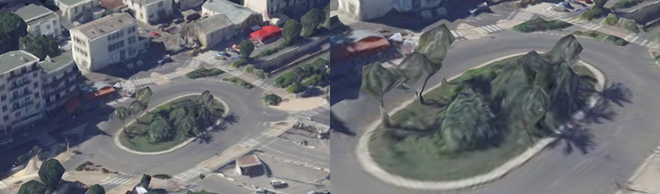
\includegraphics[width=\textwidth]{images/Stadsmiljo.png}
    \caption{Artefacts from trees that make the model less realistic at a zoomed-in level}
    \label{fig:stadsmiljo}
\end{figure}


\section{Problem statement}
Problems in this section / thesis : 
Visual inspection: This is problematic as it does not really allow for a systematic evaluation/comparison. You should at least formulate or define your own criteria, rather quantitative.
\\
This Master's thesis project belongs to the urban modelling and analysis field, a computer vision problem involving 3D computer graphics and machine learning. 
The goal of this Master’s thesis project is to examine the problem of automatic identification of objects (artefacts) in 3D urban meshes. More particularly, this project will study whether it is possible to generalise an already-existing unsupervised algorithm to lower-resolution meshes. The comparisons will be performed on datasets representing different cities and generated by different providers, with varying levels of detail and the results will be evaluated through visual inspection.  \\
The contributions of this project can be formulated as follows: 
\begin{itemize}
    \item Extending already existing semantic mesh segmentation techniques to object identification
    \item Studying the influence of mesh resolution on a state-of-the-art unsupervised mesh segmentation technique
    \item Suggestion of new geometrical features for object description in lower-resolution meshes
    \item Suggestion of an unsupervised artefact identification framework for meshes
    
\end{itemize}

\section{The Employer}
Consider removing / replacing by: it would be desirable to either include a new subsection or mention here about the scope, assumptions in the project \\ 
The employer, Carmenta, develops an advanced toolkit named Carmenta Engine to work with geospatial data, including 3D city models.  Carmenta is currently  interested  in  improving  the  quality  of  their  3D  models,  which  can  be achieved by  automatic identification of artefacts, so that they can be removed later on. 
\section{Thesis Outline}
The thesis starts with an introduction including a problem statement, followed by the Background chapter describing prior knowledge in machine learning and mesh segmentation relevant to the understanding of the thesis scientific content and placement in literature. The thesis then moves on to the Related Works chapter, presenting a more in-depth review of existing and recent literature related to the thesis content. Finally, the Methods, Results and Discussion chapters present the work carried out for this project and the conclusions drawn from it as well as suggestions for further improvements. 

\chapter{Background}
\section{Machine Learning overview}
Machine learning is a field of artificial intelligence that include a wide variety of techniques to give computers the ability to "learn" or infer models from data, without having any relationships in the data or models explicitly programmed. Machine learning techniques usually involve a training phase where the algorithms try to infer relationships or models parameters within the training data, as opposed to testing or prediction phases where the trained algorithm will predict outputs of new input data based on the learned model. \\
Supervised learning  corresponds to when the training data consists in data points $x_i$ and their respective output $y_i$. Unsupervised learning corresponds to when the training data only consists in data points $x_i$. Clustering is an example of unsupervised learning and consists in grouping a set of objects in such a way that objects in the same group, called a cluster, are more similar, according to a chosen metric, to each other than to those in other clusters.\\
Classification is when the model being learned produces discrete outputs, and the outputs are often referred to as labels. Regression is when the model being learned produces  continuous outputs, such as function estimation. \\
A feature is a one dimensional value describing part of a data point and when all features are combined into a feature vector, they then correspond to the input to the algorithm. 
\subsection{Support Vector Machines (\textcite{libsvm})} 
SVM is a supervised learning technique and non-probabilistic binary linear classifier. \\
Given a training dataset of $n$ points of the form
$(\vec{x}_{1},y_{1}),\,\ldots ,\,(\vec{x}_{n},y_{n})$ 
where the $y_{i} $ are either $1$ or $-1$, each indicating the class to which the point  $\vec {x}_{i}$ belongs. Each $\vec {x}_{i}$ is a $p$-dimensional real vector. \\
The aim is to find the "maximum-margin hyperplane" that divides the group of points $\vec {x}_{i}$  for which $y_{i}=1$ from the group of points for which $y_{i}=-1$, which is defined so that the distance between the hyperplane and the nearest point $\vec {x}_{i}$ from either group is maximized.
Any hyperplane can be written as the set of points $\vec {x}$ satisfying $\vec {w}\cdot {\vec {x}}-b=0,\,$. \\ 

In addition to performing linear classification, SVMs can efficiently perform a non-linear classification using what is called the kernel trick, implicitly mapping their inputs into high-dimensional feature spaces via kernel functions and scalar products in said higher-dimensional space. \\ 
SVMs are robust classifiers that perform well with limited amount of training data and high–dimensional data.



\subsection{Data Clustering Techniques}
\label{sec:clustering_algos}
There are fewer unsupervised learning, or data clustering, techniques present in the literature as opposed to supervised techniques. 
(\textcite{ClusteringTechniques}) presents and compares some common unsupervised algorithm on computer vision-oriented problems. 
\subsubsection{K-means}
K-means (\textcite{K-means}), minimises the sum of squared errors between data points and their
nearest cluster centres. It is a simple and widely used method. 
\subsubsection{Fuzzy C-means}
Fuzzy C-Means (\textcite{Fuzzycmeans}) assigns soft labels to data points meaning that each data point
can belong to more than one cluster with different degrees of membership.
\subsubsection{Spectral Clustering}
Spectral Clustering regroups several algorithms and is very commonly used in Data Mining for graph clustering. It consists in a spectral analysis of the matrix of point-to-point similarities instead of estimating an explicit model of data distribution (as in k-Means). Normalised Cut (\textcite{SpectralShiMalik}) and  Ng-Jordan-Weiss algorithm (\textcite{SpectralNg}) are two examples of spectral clustering algorithms. 
\subsubsection{Mean Shift}
Mean shift (\textcite{meanshift}) seeks the modes of a density function from
discrete samples of that function. Mean Shift performs as follows. First, it fixes a window around
each data point. Then, computes the mean of data within each window. Finally, shifts the window
to the mean and repeats till convergence.
\subsubsection{Deep Convolutional Neural Networks (CNNs) }
This is a description of the algorithm proposed by \textcite{ClusteringTechniques}. \\
CNNs have sparked a lot of interest recently as they have been very successful with a lot of different machine learning problems, including computer vision problems. CNNs learn representations through several stages of non-linear processing, similarly to how the cortex biologically adapts to visualise and adapt to the visual world. Such a human-perception based sounds promising as computer vision criteria often consist in human intuitions and perceptions of the results. \\
The authors use back propagation via stochastic
gradient descent to optimise a clustering objective to learn the mapping, which is parameterised by
a deep neural network. In this way, there is no need to specify parameters like number of clusters,
distance measure, scale, cluster centres, etc.




\section{Data Type}
3D point clouds and meshes can both be considered as discretised 3D functions representations. 
\subsection{3D cloud data points}
A point cloud is a collection of data points defined by a given coordinates system. In a 3D coordinates system, for example, a point cloud may define the shape of some real or created physical system. Colours can also be associated to the coordinates. \\
There are many techniques for converting a point cloud to a 3D surface.
\subsection{Mesh}
A polygon mesh is a set of vertex positions and a set of polygonal facets defined by an ordered list of vertex indices. In general, the facets are triangles. A mesh edge corresponds to a polygon edge, that is to say a segment connecting two vertices.\\
A texture is a 2D rectangular image that is being mapped onto the vertices of the mesh. Intuitively, a mesh is the 3D shape of model while the texture corresponds to a coloration of each facet. A mesh structural properties will be referred to as geometric information and properties extracted from textures as photometric information, given that the textures are usually generated from aerial pictures. 
\subsection{Comparison}
Meshes are usually created from processing of point clouds. According to \parencite{class3D},  point clouds are simple and unified structures that avoid the
combinatorial irregularities and complexities of meshes, and thus are easier to learn from. \\
Meshes generally do not enclose a volume, as they are mostly used to model surface information  for visualisation purposes whereas structures, for instance buildings, are usually characterised by a higher density in point clouds. 
\section{Mesh Segmentation}
Mesh segmentation is an active research field of geometry processing robotics and computer vision. A semantic segmentation of a mesh would be dividing it into meaningful components, following human intuition.\\

Let $M=\{V, E, F\}$ a mesh where $V$ corresponds to the mesh vertices, $E$ the mesh edges and $F$ the facets and $S$ be either $V, E$ or more usually $F$. Also called partitioning or clustering, a segmentation is a set of sub-meshes induced by a partition of $S$ into $k$ disjoint subsets. These subsets can be called regions or segments.
A mesh segmentation can usually be formulated by specifying two key elements: a function measuring the quality of a partition, eventually under a set of constraints, and a mechanism for finding an optimal partition (\textcite{MeshSegCourse}).\\



\noindent A key aspect in mesh segmentation approaches is the design of feature vectors encoding geometric and photometric information. Geometric information correspond to information contained in the mesh while photometric information correspond to information contained in the textures. There is a very wide variety of features, also called feature descriptors, signatures or shape descriptors, that can be used to design the feature vectors. 

\subsection{Region growing} 
Region growing is a method commonly used in image processing and more specifically image segmentation. Its goal is to partition an image, or in our case a mesh, by examining initial seed points, determining whether the point that are neighbours to these initial seeds should be added to the region and then iterate on the neighbours of the newly added points until there are no suitable points left to add.  \\ 
This method calls for the definition of several concepts: 
\begin{itemize}
    \item data points, or the entities we want to regroup through the algorithm,
    \begin{itemize}
        \item pixels for images.
        \item vertices or faces for meshes.
    \end{itemize} 
    \item an adjacency relationship between points, as in Fig. \ref{fig:neighbors},
    \begin{itemize}
        \item In 2D images, we can consider either Von Neumann neighbourhoods (4-connected neighbourhoods) or Moore neighbourhoods (8-connected neighborhoods). 
        \item In meshes, if we are considering vertices, then two vertices are adjacent if they are connected by an edge. If we are considering facets, then two facets are adjacent if they share an edge. 
    \end{itemize}
    \item a similarity measure to compare two points,
    \item a threshold to decide when to accept or reject a new point into a region. 
\end{itemize}

\begin{figure}[H]
    \centering
    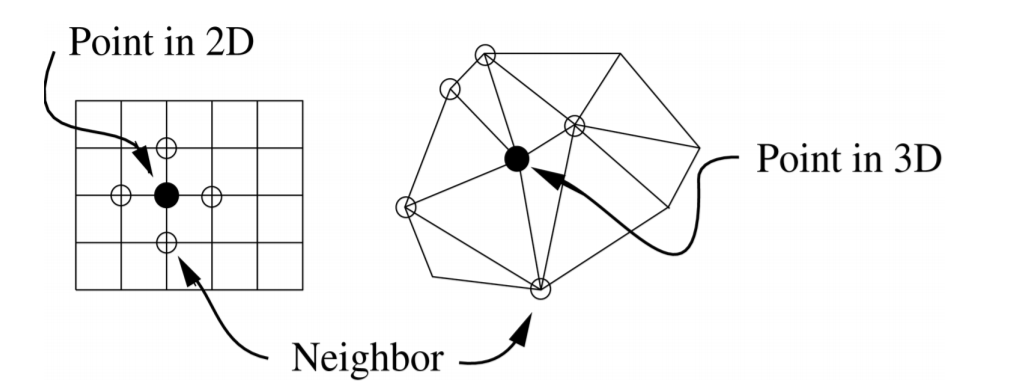
\includegraphics[width=\textwidth]{images/neighbors.png}
    \caption{Adjacency rules in 2D and in 3D, taken from \parencite{ManganMeshWatershed}}
    \label{fig:neighbors}
\end{figure}

A region growing pseudo-algorithm for the segmentation algorithm presented in \parencite{PageRegionGrowing} is then:  \\
\begin{algorithm}[H]
 \KwData{Mesh}
 \KwResult{Labels for each facet }
 initialisation\;
 \While{the mesh  not entirely segmented}{
  choose an unlabelled facet $f_0$\;
  label[$f_0$]:=k\;
  neighbours\_list:= all $f_n$ adjacent to $f_0$\;
  \While{neighbours\_list not empty}{
      $f_n$:=neighbours\_list.pop(first\_element) \;
      \If{similarity($f_n$,$f_0$) < similarity\_threshold}{
      label[$f_n$]:=k\;
      neighbours\_list.extend(all $f_i$ adjacent to $f_n$)
      }
    }
    k:=k+1
 }
 \caption{Region growing segmentation}
\end{algorithm}
\subsection{Watershed} 
Watershed is another example of techniques borrowed from image processing. It can be generalised from a 2D rectilinear grid to an arbitrary surface with well-defined neighbour connectivity, as presented in \textcite{ManganMeshWatershed} with meshes mainly. The watershed concept can also be efficiently used with 3D cloud data points (\textcite{det_seg_class} or \textcite{HernandezArtefacts}). \\
The watershed algorithm derives its name from the manner
in which regions are segmented into catchment basins. 
Let $f:X\rightarrow\mathbf{R}$ be a height function, $X$ being the set of all vertices in the mesh. Typically, $f$ can be a curvature function or a regular height function such as $f:(x,y,z)\rightarrow z$. \\

The algorithm for mesh segmentation using watershed segmentation described in \textcite{ManganMeshWatershed} has the following steps: 
\begin{enumerate}
    \item Compute the  height
function at each vertex.
    \item Find the local minima and assign each a unique
label
    \item Find each flat area and classify it as a minimum or a
plateau
    \item Loop through plateaus and allow each one to
descend until a labelled region is encountered.
    \item Allow all remaining unlabelled vertices to similarly
descend and join to labelled regions
    \item Merge regions whose watershed depth (Fig. \ref{fig:WSdepth}) is below a
preset threshold.
\end{enumerate}


\begin{figure}[H]
    \centering
    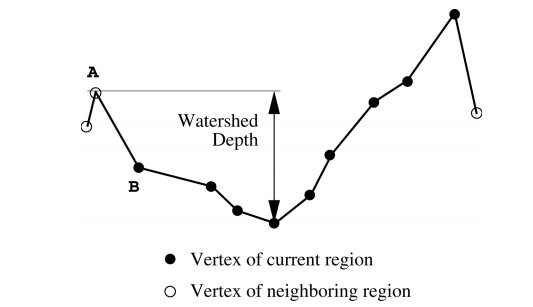
\includegraphics[width=\textwidth]{images/watershed_depth.png}
    \caption{Defining the depth of a region based on its lowest vertex and lowest boundary vertex, taken from \parencite{ManganMeshWatershed}}
    \label{fig:WSdepth}
\end{figure}

This solution strategy can be extended by bringing additional information such as triangle coloring or texture coordinate, or other saliency measures. \\ 
Although used as a mesh segmentation technique in the original article, it can also be used as an intermediate step, either for grouping similar facets as pre-processing or isolating objects, in a similar manner as in \parencite{det_seg_class}. 

\subsection{Markov Random Field} 
\label{sec:MRF}
Markov Random Fields find a wide range of applications in computer vision and machine learning, from image processing with denoising applications to semantic scene partitioning. \\

A Markov Random Field  consists in a set of random variables having a Markov property described by an undirected graph. \\
A Markov property refers to the memoryless property of a stochastic process, that is if the conditional probability distribution of future states of the process (conditional on both past and present values) depends only upon the present state; that is, given the present, the future does not depend on the past. \\ 
A MRF is always associated to a neighbourhood system
defining the dependency between graph nodes.
$N= \{n(i) \,, i \in V \}$ is a neighbourhood system if
\begin{itemize}
    \item $i \notin n(i)$
    \item $i \in n(j) \Leftrightarrow j \in n(i)$
\end{itemize}

 The markovian property and the neighbourhood system ensure that each random variable cannot be dependent to all the
other ones and reduce complexity  by spatial  considerations.
\subsubsection{MRF formulation for meshes}
Markov Random Fields for meshes
\begin{itemize}
    \item Graph nodes := vertices \& graph edges := edges
    \item Graph nodes := facets \& graph edges := edges
    \item Graph nodes := edges \& graph edges := facets
\end{itemize}

MRF formulations usually correspond to minimising an energy. The energy is commonly composed of two terms: a data term that measures the coherence of each datum with respect to a label, and a pairwise potential that favours label smoothness.
Let $G=(V,E)$ a graph and $l=(l_i)_{0\leq i < |V|} $ a label configuration for the graph nodes \\
\[ U(l)=
\underbrace{ \sum \limits_{i\in V} D_i(l_i)}_{\text{Data term} } + \gamma \underbrace{ \sum \limits_{\{i,j\} \in E} V_{ij}(l_i, l_j)}_{\text{Pairwise potential }} , \qquad \gamma>0
\]
When in a Bayesian case, $$\text{data term}=-log(\text{likelihood}) \\ \text{ and pairwise potential}=-log(\text{pairwise interaction prior})$$


MRF formulated as an energy minimisation makes it possible to use efficient algorithms to find the optimal labelling such as simulated annealing, graph-cut based approaches, Monte Carlo sampling... 
\subsubsection{MRF solving through graph cuts}
Graph Cuts finds the optimal solution to a binary problem. However when each node can be assigned many labels, finding the solution can be computationally expensive. For the aforementioned type of energy,  graph cuts can be used subsequently to find a convenient local minimum. \\
General algorithm from \textcite{BoykovEnergyMinim}: 
\begin{figure}[H]
    Let $L$ a label set and $E$ an energy function
    \begin{enumerate}
        \item Start with an arbitrary labelling f
        \item Set success := 0
        \item For each pair of labels $\{\alpha, \beta\}\subset L$
        \stepcounter{enumi}
        \begin{enumerate}
            \item Find  $\hat{f} = \text{arg  min} \, E(f')$ among $f'$ within
one $\alpha-\beta$ swap of $f$ 
            \item If $E( \hat{f}) < E(f)$, set $f := \hat{f}$ and success := 1
        \end{enumerate}
        \item If success = 1 goto 2
        \item Return f
    
    \end{enumerate}
    \caption{Energy minimisation algorithm with Graph Cuts}
    \label{fig:minim_energy}
\end{figure}


The main idea of the alpha-beta swap algorithm is to successively segment all $\alpha$ nodes from $\beta$ nodes with graph cuts and the algorithm will change the $\alpha-\beta$ combination at each iteration. The algorithm will iterate through each possible combination until it converges. \\
Within an iteration (step 3. of algorithm \ref{fig:minim_energy}), a graph (cf Fig. \ref{fig:graphCut}) is constructed: it consists in all vertices with label $\alpha$ and $\beta$, two additional terminal nodes named $\alpha$ and $\beta$. There are then two types of edges: n-links or edges between vertices (the ones corresponding to the mesh) and t-links or edges between a vertex and a terminal node. Details on the weights can be found in (\textcite{BoykovEnergyMinim}). \\
The energy of a configuration is then equivalent to the capacity of the minimum cut in the graph, and can be found through max-flow/min-cut capacity as proposed in \textcite{KolmogorovMaxflow}. \\

\begin{figure}[H]
    \centering
    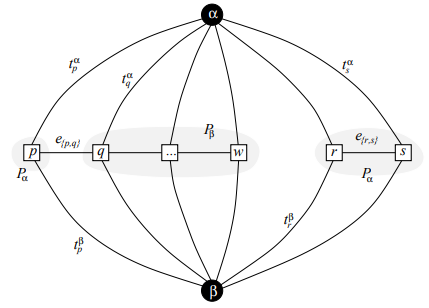
\includegraphics[width = \textwidth]{images/abgraph.png}
    \caption{Taken from \parencite{BoykovEnergyMinim}: An example of the graph $G_{\alpha\beta}$ for a 1D image.
The set of pixels in the image is $P_{\alpha\beta} = P_\alpha \cup P_\beta$  where 
\{vertices with label $\alpha$\} $=P_\alpha = \{p, r, s\}$ and \{vertices with label $\beta$\} $=P_\beta = \{q,..., w\}$}
    \label{fig:graphCut}
\end{figure}

\subsection{Metrics} 
 \textcite{Zhang2008ImageSE} provide a study on quality assessment of \textit{2D images} segmentation, classifying methods in five groups: 
\begin{itemize}
    \item \textbf{Analytical methods}. These take into account the characteristics of an algorithm such as principles, requirements, complexity, \dots
    \item \textbf{Subjective methods}. The evaluation is performed in a subjective way with segmentation results judged by a human operator. This evaluation is very biased and therefore requires a large set of objects and a large group of humans and cannot be integrated in an automatic metric evaluation. 
    \item \textbf{System level evaluation methods}. This kind of
methods indicates if the characteristics of the results
obtained by a segmentation algorithm are suited
for the over-all system which uses this segmentation
algorithm. 
    \item \textbf{Empirical goodness or unsupervised methods}. The performance of the algorithms is evaluated
by judging the quality of the segmented images
themselves. To achieve this task, a set of quality
is established
according to human intuition about what conditions
should be satisfied by an ideal segmentation. It is however difficult to specify a priori criteria for the evaluation of a segmentation quality. 
    \item \textbf{Empirical discrepancy or supervised methods}.
    A set of references images representing the ideal segmentations constitutes a ground-truth. The evaluation is then carried out by measuring the discrepancy between the ground-truth and the segmentation algorithm results. 
\end{itemize}

These categories can be extended to 3D segmentations. However, lacking a ground-truth segmentation, a lot of semantic segmentations of urban meshes are evaluated through visual inspection and designing metrics is an active research field. \textcite{ComparativeStudyMetrics} designed metrics following a set of principles for segmentations comparison. A reliable measure of mesh segmentation similarity has to possess the following set of properties: 
\begin{itemize}
    \item \textbf{No degenerative cases}. The score’s measure must
be proportional to the similarity degree between an
automatic segmentation and the ground-truth segmentations
of the same model.
    \item \textbf{Tolerance to refinement}. Some humans can provide a coarse segmentation while others will provide a finer one. The common element being that both segmentations remain consistent. Thus a segmentation measure has to be invariant to granularity differences between segmentations.
    \item \textbf{Cardinality independence}. Two segmentations compared can have different numbers of segments
and different sizes of segments. 
    \item \textbf{Tolerance to cut boundary imprecision}. The boundaries tend to vary between two similar segments and thus do not have such an importance from a semantic point of view. 
    \item \textbf{Tolerance to multiple ground-truth}.
    \item \textbf{Meaningful comparison}. The scores obtained by
the measure have to allow a meaningful comparison
between different segmentations of the same model
and between segmentations of different models. For
the first case (segmentations of the same model),
the scores have to vary according to the segmentation
quality, then, the more the automatic segmentation
is similar to the ground-truth segmentations of the
same model, and better the score is. For the second
case (segmentations of different models), the scores
have to indicate which kind of 3D-models is the most
convenient to segment by an automatic algorithm
\end{itemize}

Finally, \textcite{ComparativeStudyMetrics} categorise mesh segmentation measures into three categories:  
\begin{itemize}
    \item \textbf{Boundary matching}. This kind of measure computes
the mapping degree between the extracted region
boundaries of two segmentations.
    \item \textbf{Region differencing}. These measures compute the
consistency degree between the regions produced by
two segmentations.
    \item \textbf{Non-parametric tests.} Different non-parametric measures can be found in the statistical literature. Some of them are variants of the Rand index.  This index converts the
problem of comparing two segmentations
with different numbers of segments into a problem of
computing pairwise label relationships. The Rand index can be computed
as the ratio of the number of pairs of vertices or faces
having the compatible label relationship in both segmentations. 
\end{itemize}




% \section{Terminology}
% \textbf{Artefact or artefact}: 
% Any undesired or unintended alteration in data introduced in a digital process by an involved technique. In the thesis context, we extend the notion to unwanted objects present in the model. \\
% \textbf{Mesh}: 
% A polygon mesh
% generally consists of a set of 3D vertex positions and a set of polygonal facets each
% defined by an ordered list of vertex indices. The ordering of vertices of a facet determines
% its orientation. In this report, unless explicitly specified otherwise, facets are triangles. 
% \\\textbf{Resolution}: Intuitively how detailed and smooth the mesh looks. Related to the size and number of triangles of the mesh. 

\chapter{Related Work}
This chapter presents a review of the most recent and related works on 3D automatic analysis of urban environments, which is to say semantic segmentation with focus on methods dealing with meshes of urban scenes and objects detection in urban 3D point clouds. Even though 3D acquisition systems have reached a high maturity level, 3D automatic
analysis of urban areas is still an active research area. 

\section{Mesh and Image oriented techniques}
\subsubsection{Classification}
Image, or point cloud, partitioning in computer vision is a recurrent problem that many different classification approaches have tried to solve. In general, the aim is to partition the input data into labelled areas with criteria following a human intuition of the result. Classification approaches differ mainly in level of supervision, chosen features to extract and  use of
spatial dependencies and contextual information.  Many supervised approaches can be found through literature and \textcite{rouhani} propose a detailed and urban mesh segmentation-oriented overview of these approaches.  \\
Clustering and classification tend to be studied separately in computer vision or even machine learning in general. Neural Networks, in principle, learn from the data the same way humans do and therefore hold potential for applications with  human-oriented standards for results.  \textcite{ClusteringTechniques} propose a Deep Convolutional Neural Network (CNNs) for human-like clustering inspired after the use of CNNs in semantic segmentation problems and compare their solution to already existing clustering algorithms (presented in Section \ref{sec:clustering_algos}).. 

\subsubsection{ MRFs and CRFs}
MRFs and CRFs are preferred classification techniques for  semantic segmentation: in MRFs and CRFs, a datum classification depends on the rest of the data, as the classification decision relies on non-local information accounting for spatial consistency between neighbouring areas.  \\
Generally, the results of semantic segmentation can be improved with information derived form the context.  \textcite{Ladicky:2013:IMC:2503179.2503202} use co-occurence statistics by recording which pairs of classes are likely to occur in the same image. 
\textcite{Myeong2012} describe region pairwise relationship through a similarity graph. Finally, semantic segmentation and object detection can be improved by combining both global and local contexts 
(\textcite{Mottaghi2014}) to improve both semantic segmentation and object
detection.  

\subsubsection{Mesh segmentation}
There is a large variety of mesh segmentation algorithms in the literature, shared with image processing and computer vision fields.  One of the simplest way to deal with mesh segmentation is by representing it as an unsupervised
clustering problem based on specific geometric criteria (\textcite{Shlafman2002MetamorphosisOP}). Region growing (\textcite{PageRegionGrowing}) and spectral analysis (\textcite{ZhangSpectral}) are other examples of deterministic approaches. 
MRFs and CRFs are probabilistic approaches that help capture contextual and spatial consistency (\textcite{lafarge:hal-00759261}). These probabilistic approaches allow to have solutions  ranging from unsupervised segmentations to supervised segmentations: \textcite{verdie}  design three geometric attributes for a labelling cost function to define the unary term while  \textcite{rouhani} predict it. \\ 
Finally, Neural Networks and Deep Learning techniques have also been applied to mesh segmentation problems. \textcite{George2018} propose  Multi-Branch 1-dimensional CNNs on  11-feature vectors extracted from the input mesh. \textcite{Shu2016} perform 3D shape segmentation and co-segmentation using deep learning with the following steps: i) generation of primitive patches for each shape input; ii) extraction of  several shape descriptors from each patch and concatenate them into a resulting feature vector; iii) use the previously obtained feature vectors as input for a deep neural network in order to general a high-level feature space; iv) segmentation by performing a clustering operation in the high-level feature space.  


\subsubsection{Image-based techniques in Multi-View Stereo }
As 2D image segmentation and analysis is an important segment of the image processing literature, in MVS contexts, rather than processing the output mesh,  some methods first perform classification directly from
the images before mapping it to the output 3D model (\textcite{He2013}).  \textcite{lafarge:hal-00759261} propose a hybrid approach, refining the output model while detecting regular urban objects.    The
incremental approach proposed by \textcite{Vineet2015} operates in near real
time and delivers a rough reconstruction with a street-based semantics. \textcite{Xiao2009} propose a larger MRF that includes all the views, and
models all connections between the associated areas. The smoothness term
between two views is defined either based on the colour similarity or using
the number of common feature tracks between the two associated images.
These image-based methods are compute-intensive and insufficiently exploit
the geometric properties of the observed scene (\textcite{rouhani}).

\section{Point cloud oriented techniques}
ALS: Aerial Laser Scan; \\
MLS: Mobile Laser Scan; \\
TLS: Terrestrial Laser Scan; 
\subsubsection{Elevation images}
Point clouds are usually very dense and their processing lead to high computation time and complexity. Therefore, 3D information is commonly projected onto a 2D grid. When the information contained in each pixel corresponds to elevation information, the grid is commonly referred to as range or elevation image, or digital elevation model. These 2.5D images have a long tradition in the scientific community (\textcite{Hoover1996}) and are still of interest due to technological advances in remote sensing, with the Kinect for instance (\textcite{SaponaraIriartePaniagua654209}). 
\textcite{Gorte2007PlanarFE}
presents a method to segment planes on TLS data using range images. They obtain a so-called panoramic range image and estimate planes for each pixel of the image. They then regroup pixels belonging to a same plane through region-growing.  \textcite{HernandezArtefacts}, improved later on by \textcite{det_seg_class} propose a solution with the following steps: i) projection of 3D point cloud to elevation images; ii) ground segmentation through $\lambda$-flat zones algorithm (\textcite{morphoMeyer}); iii) object detection based on mathematical morphology transformations; iv) object classification using an SVM classifier.  

\subsubsection{Real-time applications and autonomous driving}
Real-time applications favour elevation images processing as it is both precise and fast. Falling in that category, 
approaches for autonomous vehicles generally  require average accuracy and high speed in order to detect and predict obstacles in real
time. Recent LIDAR-based methods place 3D windows
in 3D voxel grids to score the point cloud \parencite{zengang2015, vote3deep2016} or apply
CNNs to the front view point map in
a dense box prediction scheme \textcite{BoLi2016}. Image-based methods
\parencite{Chen2016, Chen2} typically first generate 3D box proposals and then perform region-based recognition.  Methods based on LIDAR point cloud
usually achieve more accurate 3D locations while image-based
methods have higher accuracy in terms of 2D box
evaluation.  \textcite{autonomous_driving} combine LIDAR and images for 3D
detection by employing a deep fusion scheme.



\subsubsection{General semantic segmentation}
Several general segmentation and classification frameworks can be also
found in the literature. \textcite{Golovinskiy2009} develop a set of algorithms
to detect, segment, characterise and classify urban objects.  Their pipeline is
as follows: i) ground segmentation using graph cuts, ii) object detection
and segmentation using hierarchical clustering, iii) object characterisation
using geometrical and contextual descriptors, and iv) object classification
using SVM. More recently, \textcite{Velizhev2012ImplicitSM} have improved this workflow
including spin images and implicit shape models. The major problems of
these approaches are noise, sparse sampling and proximity between objects.
Moreover, some prior knowledge about the object scale is required to set up
thresholds. \\
\textcite{Schnabel2012} present a semantic system for 3D shape
detection. Their algorithm consists in two main steps: i) a topology graph
is built with primitive shapes extracted from the data; ii) a search is carried
out in order to detect characteristic subgraphs of semantic entities. The
main drawback is the graph complexity when dealing with non-trivial objects.
\textcite{PU2011S28} propose a framework for segmenting and classifying
urban objects from MLS data. This work starts with a rough classification
into three large categories: ground, on-ground objects and off-ground objects.
Then, based on geometrical attributes and topological relations, more
detailed classes such as traffic signs, trees, building walls and barriers are
recognised. \\


\section{Urban modelling}
3D urban analysis is a topic which is often included in urban modelling or urban reconstruction, which regroups a high volume of literature entries while still facing many unsolved problems (\textcite{UrbanReconstructionSurvey}): extracting semantics from the input data is an important and challenging step of urban reconstruction. The classes of interest generally consist in stationary elements such as buildings, roads or eventually trees. \\
\textcite{RottensteinerSurvey} provide a comprehensive survey on both 3D urban reconstruction and  urban object classification (2D outlines of
urban objects in the input data).   Non-local strategies exploiting spatial and contextual information in urban scenes have proven rather efficient, both on images (\textcite{Volpi2015, MontoyaZegarra2015SemanticSO}) and on 3D point clouds (\textcite{Lai2014, NIEMEYER2014152}). \\
Trees are a special object of focus for urban modelling as it is usually complicated to capture their shape and usually results in complex models calling for simplification. \textcite{Rutzinger2011} describe an automated workflow to
segment and model trees from MLS data: i) input point cloud is segmented into planar regions using the 3D Hough Transform and surface growing algorithms; ii) remaining small segments are merged through connectivity analysis; iii) non-tree objects are excluded from
the analysis; iv) trees are thinned  and realistic 3D models are 
generated. \textcite{Finnish3Dpc} propose an algorithm for urban 3D segmentation and modelling from street view images and Lidar point clouds. Their proposal for urban segmentation is the following: they first isolate road points from the point cloud by locally computing minimum z-values and then performing plane fitting on the lowest points; then, they segment the building façades through a rule-based segmentation using height and density features.  They then use a boosted decision tree detector for super-voxel
features to classify the different objects present in the remaining point ensemble. \\
Literature on analysis of urban meshes is more marginal. \textcite{verdie} segment an input mesh into four classes: ground, facades, roof and vegetation. This unsupervised classification relies on three geometric features: elevation, planarity and verticality used in labelling cost function modelling the unary term of a MRF.  \textcite{rouhani} propose a supervised approach based on \textcite{verdie} geometric features and introduce a joint-labelling strategy as well as photometric features. \textcite{martinovic2015} use a supervised classifier modelling a labelling cost function. They also use a corrective post-processing step. 









\chapter{Methods}
The iterature on object detection in meshes is rather marginal. Therefore, the present work suggests a solution adapted from object-detection-and-classification algorithms on point clouds (\textcite{HernandezArtefacts, det_seg_class} or \textcite{Finnish3Dpc}). 
The suggested algorithm pipeline will have the following steps: \\
Maybe use a chart here
\begin{center}
\begin{enumerate}[topsep=2ex,itemsep=-1ex,partopsep=1ex,parsep=1ex]
    \item Pre-processing
    \item Primary clustering (Ground detection)
    \item Post-processing
    \item Objects detection
    \item Objects classification
\end{enumerate}
\end{center}

The input data corresponds to an urban textured mesh. 
\section{Pre-processing}
This section covers computations performed at the beginning of the pipeline, either in order to achieve better consistency in measures, reduce computation time or to gather information about the whole mesh. 
\subsection{Connectivity analysis}
Meshes are usually unified and internally-connected structures. However, it is rather common for automated reconstruction methods to fail to capture certain details leading to the presence of disconnected components within the mesh. \\ 
The general idea is then to perform region growing on the triangles, with adjacency being the only constraint. To be considered adjacent, two triangles must share an edge. The algorithm result then consists in all of the connected components present in the mesh. Whether a cluster of triangles should be considered as unwanted is then decided based on comparing the number of triangles contained in the component to an arbitrary threshold. \\
There are several things that should be kept in mind while conducting such a connectivity analysis, depending mainly on the reconstructed model. If the acquisition and triangulation methods are precise enough, the resulting model might not contain any disconnected components. When the model contains different levels of detail, higher levels of detail can correspond to such disconnected component, and therefore do not need to be removed. Finally, it is common during the data acquisition and the reconstruction steps to process smaller areas or tiles one at a time. One direct implication is that objects at the border between two areas might be divided in two separate groups only matching visually. 
\subsection{Division into sub-meshes}
Urban meshes modelling an entire city contain a lot of triangles and direct processing of the entire model would lead to unpractical computation time and memory requirements. The original mesh is therefore divided into smaller meshes.  \textcite{HernandezArtefacts} separate city blocks using the Hough transform to detect façades direction, under the assumption that the façades of a same street are aligned. This assumption is however not always verified across the datasets used for this work. \\
The only considerations for this division are memory and computation time reduction, therefore the mesh is divided into arbitrary-sized rectangular meshes, judged large enough to contain semantic information about large structures such as buildings. 
\subsection{Elevation and density maps}
This step is actually performed before dividing the original mesh into sub-meshes. It is useful either in order to obtain an elevation image and perform a mathematical morphology-oriented strategy as in \parencite{det_seg_class, HernandezArtefacts} or to help compute the elevation and density features for the mesh segmentation strategy. For the latter, computing values before division of the mesh ensures consistency near the separation lines.  
\subsubsection{Elevation image}
The following paragraphs describe how to get an elevation image from the mesh vertices. Unlike point clouds, mesh vertex ensembles are sparse and would not be enough to estimate surfaces without the additional information provided by the faces. Therefore, in an attempt to adapt point cloud solutions to meshes, additional vertices need to be generated. One way is to sample new vertices from triangles according to the grid we want to project the vertices on and the constrained plane equation defined by a triangle. \\
We consider the rectangle bounding the projection of the triangle $T$ on the XY plane (in red in figure \ref{fig:vertices}). For each grid point $(i,j)$ contained in the bounding rectangle, if $(i,j)$ is within the projection of the triangle, then a new vertex $v_{new}=(i,j, z_{new})$ is created from the equation of the plane passing through $T$ (the plane is defined by the triangle normal and one vertex from the triangle). One can determine whether a point is inside a triangle using a barycentric coordinate system in the triangle: \\ 
A point $(p_x, p_y)$ is in triangle $T= \{ (v_{0x},v_{0y} ), (v_{1x},v_{1y} ),(v_{2x},v_{2y} )\} $ \\
$\iff \forall x_i \text{ in } x, x_i \geq 0 \text{ with $x$ solution of } Ax=b$ \\
where $  A = \begin{bmatrix}
        v_{0x}  & v_{1x} & v_{2x}    \\
    v_{0y} & v_{1y} &   v_{2y} \\
    1  & 1 & 1
\end{bmatrix} $ and $b = \begin{bmatrix} p_x \\ p_y \\ 1 \end{bmatrix}$ \\

Once the vertices are obtained, they are projected onto the grid similarly to \parencite{det_seg_class} and we obtain two arrays: one for the minimal height in a local neighbourhood represented by the grid resolution and another one for the maximal height in the same local neighbourhood. 

\begin{figure}
    \centering
    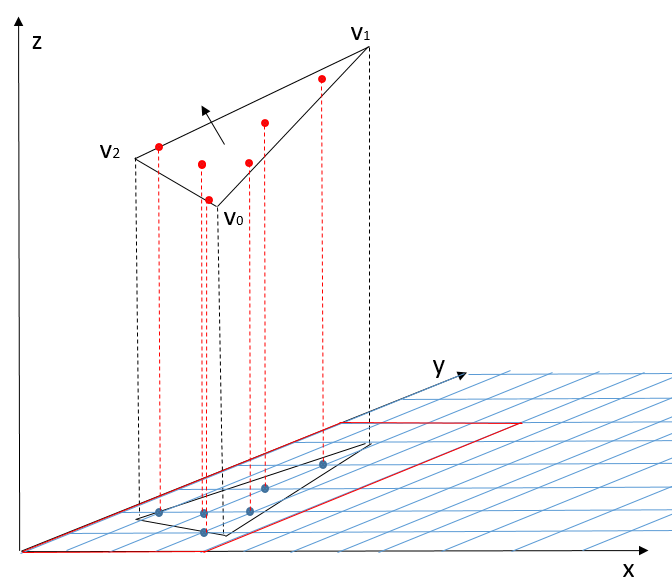
\includegraphics[width=0.7\textwidth]{images/vertices_sampling.png}
    \caption{New vertices generation from triangle sampling}
    \label{fig:vertices}
\end{figure}

\subsection{Superfacet partitioning}
As input meshes are very dense, labelling each facet requires a lot of computations and leads to impractical computation times with an MRF formulation. Superfacet partitioning \parencite{rouhani, verdie} consists in grouping facets into small clusters, an over-segmentation analogous to superpixels in image analysis. \\
Clustering is performed through a region growing approach over all triangles based on a similarity measure. A region grows until the similarity measure exceeds a user-specified threshold. Additionally, a constraint on superfacet areas can be formulated. \\
In a lot of applications, choosing a similarity measure and the corresponding threshold corresponds to the challenging part. The following sections present different choices for similarity measures.
\subsubsection{Shape operator}
The shape operator is a measure of how a regular surface bends in $\mathbb{R}^3$. Evaluated at a point on a surface, it is a linear transformation of the tangent space that measures how the surface bends in different directions \parencite{ShapeOpBook}. The normal curvature of a surface in some direction
is the reciprocal of the radius of the circle that best approximates
a normal slice of surface in that direction. \\
\textcite{curvPaper} provides an algorithm for the estimation of the curvature and the second fundamental form, whose matrix formulation is the same as the shape operator's. This estimation method outperforms Cohen-Steiner and Morvan algorithm \textcite{CohenSteiner:2003}, used by \textcite{verdie}. \\
This metric identifies the nearly planar components and preserves sharp features. Comparison can be performed via the Frobenius norm on the estimated second fundamental form matrix. 
\subsubsection{Normal comparison}
Used in \textcite{rouhani}, \textcite{CohenSteiner:2004} introduce $\mathcal{L}^{2,1}$ as Shape metric. It is essentially an $\mathcal{L}^2$ measure of the normal field: 
$$\mathcal{L}^{2,1}(R_i, P_i)= \iint \limits_{x \in R_i} ||\mathbf{n}(x) - \mathbf{n}_i||^2dx$$
with $R_i$ a region of a partition and $P_i=(x_i, \mathbf{n}_i)$ a planar proxy passing through $x_i$ with normal $\mathbf{n}_i$ approximating $R_i$. \\

Intuitively, normal orientation and co-planar regions give a lot of information on the structure of an object. The previously explained measure can simply amount to a normal comparison during region growing, with the threshold being a maximum angle: a facet is admitted if the angle difference between its normal and the average normal of the region is smaller than the threshold. 
\subsubsection{Colour comparison}
Jointly used in \textcite{rouhani} with the covariance-based shape estimator from \textcite{CohenSteiner:2004}, photometric information helps preserving image discontinuities of the texture map. It is computed as the L1-distance in the colour space. Colours help us perceive the boundaries of objects and recognise some of them, trees for instance are characterised by green tones. Therefore, if available, trying to use photometric information for clustering similar facets follows human intuition and perception. 


\section{Primary clustering}
This section mainly presents two suggestions for ground detection in a sub-mesh. The first one is an adaptation of a point cloud strategy adopted in \parencite{HernandezArtefacts, det_seg_class} to meshes. The second one extends \parencite{verdie} to meshes with varying resolutions, as it struggles with tree detection as the mesh resolution decreases. 
\subsection{Feature extraction}
\label{sec:ft_extract}
In order to capture the information contained in triangles or the mesh in general, features must be computed. They are used mainly for triangles labelling in the mesh segmentation approach but were also used for vertices clustering in the adaption of the point cloud approach. Elevation, planarity and horizontality (or verticality) were first introduced by \textcite{verdie}. \\ 
When using superfacets, for each superfacet, the feature value is  the area-weighted sum of the feature value
of its triangle facets.
\subsubsection{Elevation}
Elevation discriminates the ground from higher objects
such as roofs. It measures the height of a point with respect
to the ground. 
$$\text{Elevation}(p(x,y,z)) = \sqrt{\frac{z - z_{min}(x,y)}{z_{max}(x,y)- z_{min}(x,y)}}$$
where $z_{min}$ and $z_{max}$ are respectively the minimal and maximal z-coordinates in a local window on the XY plane and z is the z-coordinate of the point. If we are looking at facets, $z$ is the z-coordinate of the barycenter of the triangle. \\
The $z_{min}$ and $z_{max}$ are pre-computed during pre-processing. The size of the local window must be large enough to meet ground areas and small enough to offer robustness to terrain height variation. Using open source data such as Open Street Map, the window sizes could be estimated automatically based on buildings dimensions: the window size $L$ such that the window has an area of $L\times L$ should be larger than the smaller dimension of the larger building bounding rectangle in the scene. 

\subsubsection{Planarity}
Planarity was derived from the surface variation introduced by \textcite{Pauly2002}: it is computed from the minimum eigenvalues of the covariance
matrix computed in closed form over all triangle facets of the
superfacet and measures how much the superfacet deviates from the local tangent plane, yielding 1 for planar superfacets and 0 for isotropic superfacets.  \\
In order to get a facet-oriented measure, this work suggests for planarity measure the average cosine angle between a facet normal and its neighbouring facets unit normals:
$$\text{Planarity}(t)= \frac{1}{|\mathcal{N}(t)|} \sum \limits_{t_i \in \mathcal{N}(t)}  |\mathbf{n}(t) \cdot \mathbf{n}(t_i)| $$ where $\mathcal{N}(t)$ is the neighbourhood ensemble of a facet $t$. \\
In \textcite{verdie}, planarity is used to discriminate vegetation from the other three classes: roof, façade, ground. However, this feature might not be very efficient for lower-resolution meshes for tree identification. 

\subsubsection{Horizontality}
This feature measures the deviation of the unit normal $\mathbf{n}$ of a facet to the vertical axis $\mathbf{z}$: 
$$\text{Horizontality}=|\mathbf{n} \cdot \mathbf{z}|$$
A low horizontality value corresponds to vertical components, which corresponds to façades mainly. A high horizontality value corresponds to horizontal components, typically roofs and roads. 

\subsubsection{Density}
This feature comes from analyses performed on point clouds: LiDAR reconstructions provide dense and high regions for building façades \parencite{Finnish3Dpc}. In meshes, façades and trees lead to a higher number of triangles in a small window of the XY plane while flat areas are usually sparse in terms of triangles and vertices. \\ 
In the pre-processing part, vertices are assigned to $1m\times1m$ areas. The resulting vertices count array is then clamped and normalised. The clamping rule is the following: \\

\textbf{if} vertices\_count[i,j] > mean(vertices\_count) + $\sqrt{\text{variance(vertices\_count)}}$ \\
\textbf{then} vertices\_count[i,j]=mean(vertices\_count) + $\sqrt{\text{variance(vertices\_count)}}$\\

Which results in a value close to 0 for sparse areas and close to 1 for areas with a high number of vertices. 
\subsubsection{Greenness}
This feature also intends to discriminate trees from other components. Greenness corresponds to how green a triangle is, computed from the Hue value in Hue-Saturation-Value (HSV) colour space. HSV space describes colour in way that is similar to human perception. The Hue value corresponds to an angle on the chromatic circle, on which green is represented by 120\degree. In computer vision, the sensibility $s$ for a colour perception is commonly 30-40\degree around the colour. This yields: \\
$$\text{Greenness}(\text{Hue}, s)=\frac{|\text{Hue}-120|}{s} \mathbbm{1}_{|\text{Hue}-120|)<s} $$
Identifying tree triangles based on their colours feels rather intuitive, although not systematic as trees are quite obviously not stationary and depending on when the acquisition was performed, they might not be green. This feature is however a rather simple way to use texture information in an unsupervised approach. 
\subsubsection{Photometric features}
The photometric information contained in textured
meshes provide complementary clues for facet classification. HSV space is usually preferred over RGB space as it is more effective to discriminate objects with different reflectivity properties. \textcite{rouhani} use photometric features in HSV space, designed for each superfacet:
\begin{itemize}
    \item the average colour,
    \item the standard deviation of its colour distribution,
    \item discretised colour distribution by clustering HSV colour values of the whole texture map into a color palette \parencite{color_palette}.
\end{itemize}
\subsection{Elevation map and mathematical morphology strategy adaptation}
This section is inspired by the elevation map approach in \parencite{det_seg_class, HernandezArtefacts}. Their strategy for ground segmentation is based solely on elevation images and morphological operations on the images. Unlike point cloud, urban meshes are mostly surface representations and therefore discriminating maximal and minimal elevation images can not be generated from them. Adapting a point cloud approach hence also means adapting its use case: here, the elevation map is intended for road and planar areas discrimination from buildings. Then, having this ground model, object detection can be performed on triangles present in this model.  
\subsubsection{$\lambda$-flat zones labelling algorithm}
Based on \textcite{morphoMeyer} labelling algorithm in image processing, \parencite{HernandezArtefacts, det_seg_class} obtain the ground mask as the largest $\lambda$-flat zones (Definition 1) in the elevation image. \\

\textbf{Definition. } \textit{Let f be a digital gray-scale image } $f:D \subset \mathbb{Z}^2 \rightarrow V = [0, \dots, R] $. \textit{Two neighbouring pixels p,q belong to the
same $\lambda$-flat zone of $f$, if their difference
$|f_p - f_q|$ is smaller than or equal to a given $\lambda$ value.} \textit{$\forall x \in D$, let $A_x(\lambda)$ be the $\lambda$-flat zones of image f containing pixel x.} \\
$A_x(\lambda) = \{x\}\cup \{q| \exists P=(p_1=x, \dots, p_n=q) \, such \, that \, |f_{p_j}-f_{p_{j+1}}| \leq \lambda \}$\\

With this definition, the ground mask $g_m(f)$ is $g_m(f) = \text{arg} \, \max \limits_{x \in D}(|A_x(\lambda)|$. \\ 

In the eventuality of a finely captured mesh, this approach can be used as such to generate the ground mask. However, as the resolution decreases, the ground disappears under large objects such as trees. This has for effect to stop the region growing in the middle of the role and to have several $A_x(\lambda)$ corresponding to the ground. \\ 
In order to choose relevant regions, it is possible to look for local minima in the elevation image and  consider regions containing these minima. \\
Optionally, the resulting ground mask can be smoothed via morphological closing. 

\subsubsection{Clustering pixels using k-means}
Alternatively to using region growing via $\lambda$-quasi-flat zones, it is also possible to cluster the pixels of the elevation image using features computed from triangles mapped to the image: elevation and horizontality. Once k-means is performed, the cluster centre with the minimal elevation corresponds to the ground label. The ground mask is then all pixels having the ground label. Finally, k-means can be used in both superfacet- and a facet-oriented approaches.

\subsubsection{Backprojection}
Backprojection consists in going from the binary image to labelled triangles. Triangles mapped onto the ground mask pixels are labelled as ground (and the other ones as 'other'). However, some pixels might contain façades triangles and in order to label them correctly, an additional clustering, similar to the one applied on pixels, separates ground triangles from façades triangles: minimal horizontality corresponds to façades and minimal elevation to the ground.  \\


\subsection{Unsupervised triangles classification}
Directly labelling triangles corresponds to a mesh segmentation approach. 
\subsubsection{Clustering using k-means}
Clustering triangles using k-means is fast and only requires to extract features from the triangles as introduced previously. k-means also allows a flexible use of features and works in a predictable way and semantic classes labels can be inferred from the cluster centres. The predicted classes however are dependent on the data to be clustered and non-representative sub-meshes might lead to errors in the expected results. 
\subsubsection{Clustering using MRF}
An MRF with pairwise interactions formulation is a more complicated approach than k-means, but it also corresponds to a more guided and comprehensive approach: by designing unary terms similarly to \textcite{verdie}, classes formulation does not depend on the data while providing contextual and spatial consistency. Such an approach however raises the problem of how well features and unary terms can represent the desired classes. \\
Four classes are considered: $\{fa\textit{ç}ade, roof, vegetation, ground\}$.
Using the same notations as in Section \ref{sec:MRF}, the energy of a label configuration on superfacets can be written as: 
\[ U(l)=
\sum \limits_{i\in S} D_i(l_i) + \gamma  \sum \limits_{\{i,j\} \in E} V_{ij}(l_i, l_j) , \qquad \gamma>0
\] 
where S denotes the set of superfacets and E denotes all pairs of adjacent superfacets, which is to say superfacets sharing at least one edge in the input mesh. \\
The data term D combines the previously-described features weighted by the area $A_i$ of the superfacet i. \\
We refer to planarity as $a_p$, horizontality as $a_h$, elevation as $a_e$ , density as $a_d$ and greenness as $a_g$ and $\overline{a} = 1 - a$.
$$
D_i(l_i) = A_i \times  \left\{
    \begin{array}{lll}
        1 -  \overline{a_e} \cdot a_p \cdot a_h  \cdot \overline{a_d}& \mbox{if } l_i=ground \\
        1 -   \overline{a_p} \cdot a_h  \cdot a_d &  \mbox{if } l_i=vegetation   \\
        1 -   a_p \cdot \overline{a_h}  \cdot a_d & \mbox{if } l_i=fa\textit{ç}ade \\
        1 -  a_e \cdot a_p \cdot a_h  \cdot \overline{a_d} & \mbox{if } l_i=roof
    \end{array}
\right.
$$
The vegetation unary term can also be formulated as : $ 1 -   \overline{a_p} \cdot a_h  \cdot a_g $. \\
The pairwise interaction V between two adjacent
superfacets i and j favors label smoothness: 
$$V_{i,j}(l_i, l_j)=C_{i,j} \cdot w_{i,j} \cdot \mathbbm{1}_{\{l_i \neq l_j\}}$$
where $C_{ij}$ is the sum of interface (mutual)
edge lengths between superfacet i and j.   $w_{ij}$ is a weight introduced to prevent label propagation over sharp creases and is defined as
the angle cosine between the estimated normals of two superfacets. As the transition between roof and ground is judged impossible, it has a fixed high cost. Such a measure offers additional robustness for the elevation feature when encountering large flat areas. \\
As the unary data term and pairwise potential are weighted by the
superfacet areas and interface lengths, this energy formulation behaves
similarly to a triangle facet-based energy with grouping constraints.
An approximate solution to this energy minimisation problem
is solved through the $\alpha-\beta$ swap algorithm (\textcite{BoykovEnergyMinim}). 


\section{Post-processing rules}
Post-processing rules play a dual role. In the event of completely unsupervised methods, these rules correspond to the inclusion of the human rationale. They also help achieve a smoother and more inclusive ground mesh, in order to facilitate the object detection step. 
\subsection{Surrounding rule}
This rule has smoothing and consistency-enforcing motivations: if all neighbours of a triangle $T$ have the same label $l_n$ and the label of $T$ is $l_T \neq l_n$, then the label of T is changed to the label of its neighbours. 
\subsection{Watershed rule}
This rule makes sure the ground label contains all lower triangles. It also smooths the ground mesh in a watershed-like manner: if a triangle are ‘below’ a ground triangle, then they are ground triangles as well. \\
\textbf{Definition.}$t_1 \text{ below } t_2 \iff \text{PointOfMass}(t_1).z < \text{PointOfMass}(t_2).z$


\subsection{\textcite{verdie} semantic rules }
Two types of errors frequently
occur when dealing with complex urban scenes: structures on top of roofs such as chimneys often get mislabelled as vegetation and vertical components in large vegetation components get mislabelled as façades. 
\begin{itemize}
    \item \textbf{Rule 1.} Superfacets labelled as vegetation and adjacent to only superfacets labelled as roof are re-labelled as roof. 
    \item \textbf{Rule 2.} Superfacets labelled as façade and adjacent to superfacets labelled as vegetation and ground are re-labelled as vegetation.
\end{itemize}
\section{Objects detection}
The previous steps segmented an over-inclusive ground mesh from the input sub-mesh. For the two following steps, it is critical for this ground mesh to be correctly segmented. Additionally, if the previous steps are perfectly calibrated and executed, then the ground mesh should only include small objects close to the ground. 
For this section, analogously to \textcite{HernandezArtefacts}, artefacts, or objects, are assimilated to humps on the ground. The suggested method to detect and segment them is a constrained watershed from local maxima, based on a height function and additional similarity criteria. \textcite{ManganMeshWatershed} propose insights for watershed on surface meshes. In essence,  constrained watershed on meshes is growing regions whose seeds  are local maxima and with constraints both on height and similarity. The height function used here is simply the z-coordinate of a point: $\text{height}(x,y,z) = z$. It was chosen over alternative height functions such as curvature as it is easier to expect results and anticipate problems.   \\

\textbf{Definition. }$ A \, vertex\, v\, is\, a\, local \,maximum \\\iff v.z > w.z, \forall \, vertex\, w \,connected \,to\, v \,by \,an\, edge \,(of \,a\,triangle)$ \\

For the watershed, local maxima are used as markers and one marker will correspond to one object. Under the assumption that one triangle should belong to only one object at a time, rules are introduced to implement this rationale: 
\begin{itemize}
    \item If two local maxima are connected by an edge, they correspond to the same object. 
    \item All triangles connected to a local maxima are considered part of the object. Let's refer to them as seed triangles. 
    \item If two seed triangles from two different objects are adjacent, the two objects are merged into one (Fig \ref{fig:ws_merging}). 
\end{itemize}
In simple cases, where the ground is flat, segmenting objects is similar to \parencite{HernandezArtefacts}: from a marker, the object corresponds to all triangles below that marker until the ground is met.  However, on sloping ground, the height constraint is no longer sufficient when a labelled ground is not available (Fig \ref{fig:ws_angles}). Constraints based on angle changes between two adjacent triangle normals would also fail to completely capture certain types of objects such as cars (Fig \ref{fig:ws_angles}). Therefore, the suggestion for propagation constraint is the correlation distance between colour distributions of two triangles. \\
The correlation distance between $u$ and $v$ is defined as:
    $$correlation(u,v)=1-\dfrac{(u-\overline{u})\cdot(v-\overline{v})}{||u-\overline{u}||_2\cdot||v-\overline{v}||_2}$$
Colour distributions approach the human intuition perception of an object limits based on texture information:  colour helps the visual system  analyse complex images more efficiently, improving object recognition, and is commonly used in computer vision problems \parencite{hist_intersection}. 
The correlation distance is a common way to compare histograms, the discretised representation of distributions. 

\begin{figure}[t!]
    \centering
    \begin{subfigure}[t]{0.5\textwidth}
        \centering
        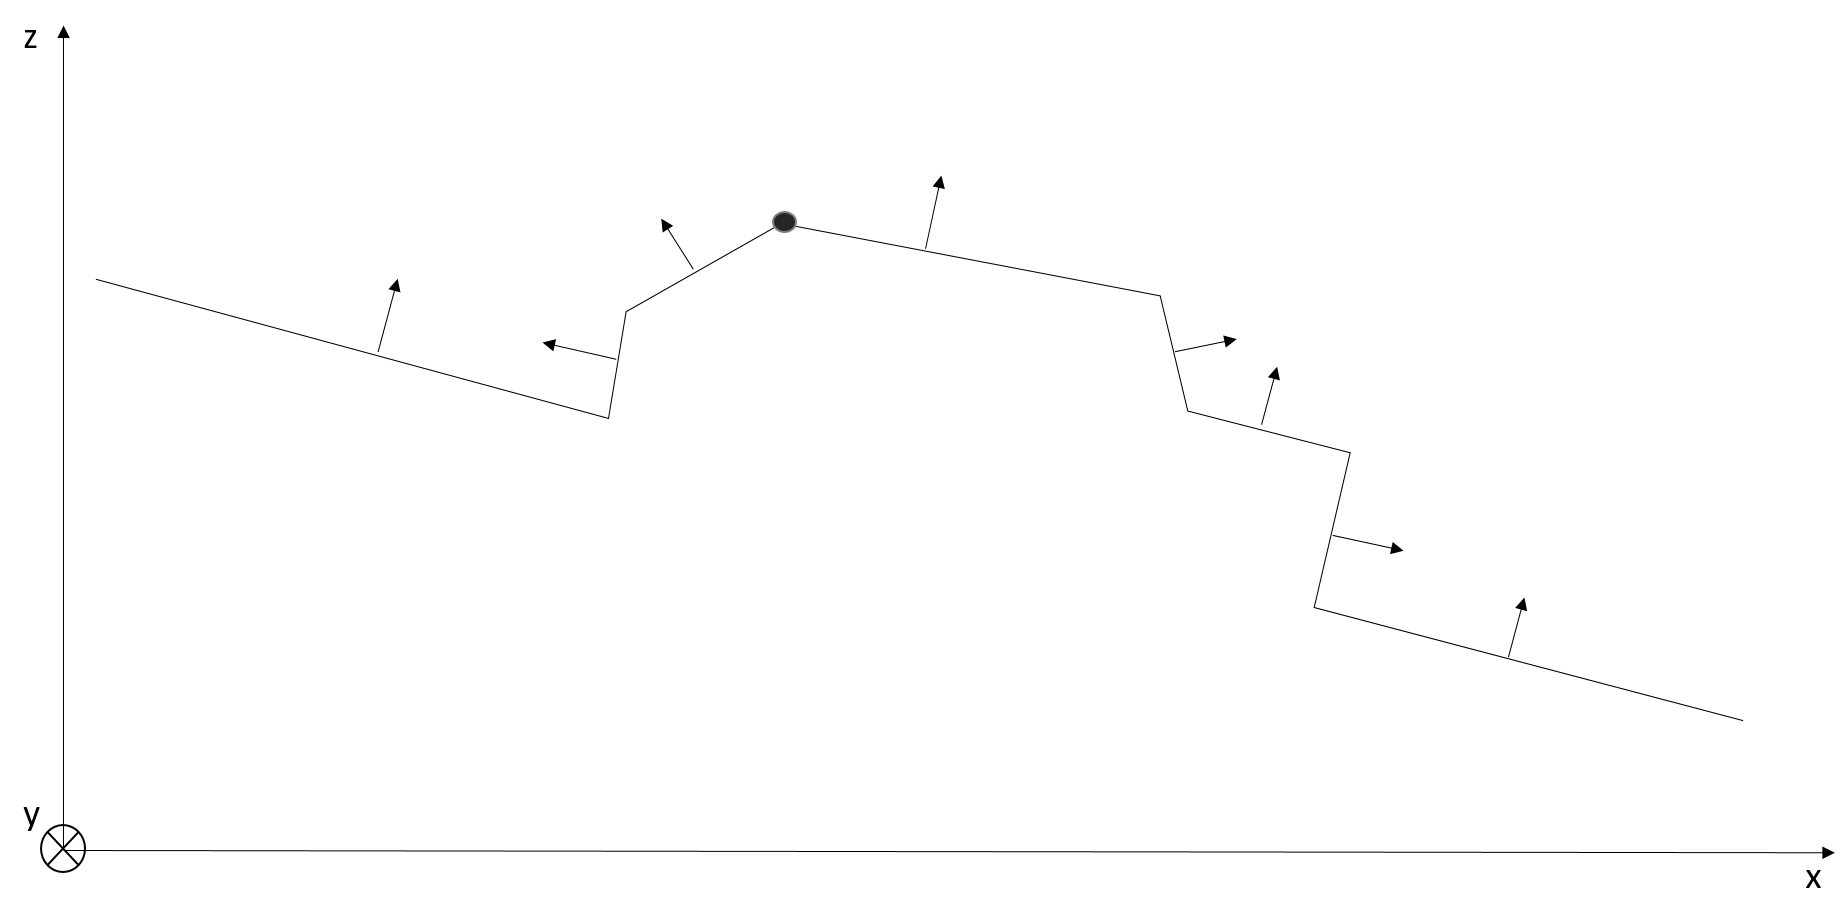
\includegraphics[width=\textwidth]{images/angles_constraint.png}
        \caption{Car profile on sloping ground }
        \label{fig:ws_angles}
    \end{subfigure}%
    ~ 
    \begin{subfigure}[t]{0.5\textwidth}
        \centering
        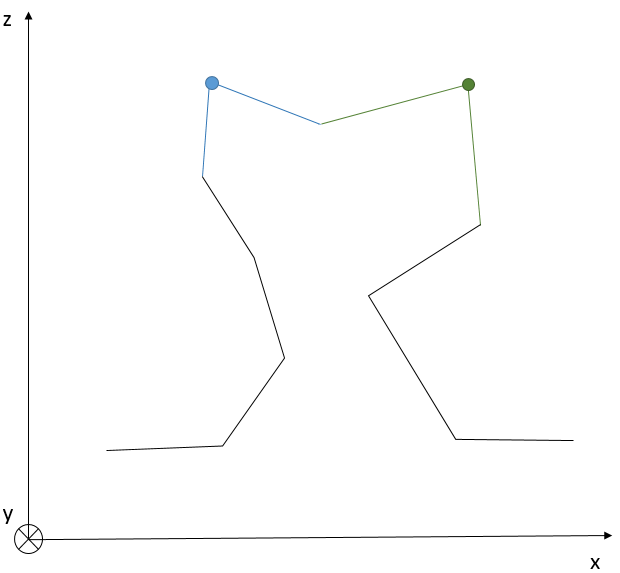
\includegraphics[width=0.4\textwidth]{images/merging_markers.png}
        \caption{A case of two markers corresponding to one object}
        \label{fig:ws_merging}
    \end{subfigure}
    \caption{Watershed for object detection. Local maxima are represented as dots}
\end{figure}


\section{Object categorisation}
Research has been carried out on mesh objects supervised classification and has proven efficient [PUT A REF HERE]. However, it was not possible due to the thesis context and schedule to generate and label manually a large and representative enough set of objects. In the eventuality of the presence of labelled  data, the classification approach could be using an SVM classifier with features similar to those used in \textcite{det_seg_class}, adapted to meshes. \\ The proposed approach is more oriented towards an engineering way to deal with the humps: by flattening them. The borders of the mesh contain local maxima and therefore objects often corresponding to lower chunks of façades. In order to prevent flattening these, a clustering based on both elevation and horizontality features using k-means is chosen. 
\section{Evaluation + Implementation }
Important part, needs to be elaborated on
\chapter{Results}
\subsubsection{Implementation}
The work was implemented in Python using Carmenta Engine to process the 3D models, OpenCV for textures processing, Networkx for graph structures and min-cut implementation and Sklearn for clustering purposes.  
\subsubsection{Datasets}
For this report, four datasets coming from three different providers were used. Bastia and Paris datasets were generated using Acute3D and aerial mapping technology by Ubick \parencite{acute3D}. Marseille dataset was generated using Pixel Factory \parencite{pixel_factory}, a Data Management and Processing Software by Airbus. Finally, Helsinki dataset is an open source 3D city model of Finland's capital \parencite{helsinki}. \\
In terms of quality of reconstruction, based on average size of triangles and overall aspect, Marseille and Helsinki datasets have finer resolutions than Paris and Bastia. 


Bastia:  \\ 
860.468831999749  x  333.57112799991387 \\
481442 \\
edge length DescribeResult(nobs=1444326, minmax=(0.0, 80.21069222735858), mean=2.8787873645898996, variance=4.522909319961517, skewness=6.810904169096826, kurtosis=145.58510413988859) \\ 
area DescribeResult(nobs=481442, minmax=(3.9519004981862886e-07, 2159.113113446979), mean=4.652083846016285, variance=197.99970316784353, skewness=76.13491963092542, kurtosis=8258.515873876877) \\ 

Paris: \\
1160.492832000234  x  1531.6114079999877 \\
triangles 809944 \\
edge length DescribeResult(nobs=2429832, minmax=(0.0, 47.251425108869384), mean=3.9626740907233358, variance=6.656769851824518, skewness=1.6776100558389642, kurtosis=6.3174207941997995) \\
area DescribeResult(nobs=809944, minmax=(0.0, 457.50438867621426), mean=8.398322162233178, variance=76.04644604507321, skewness=5.742085123391964, kurtosis=80.62966547648544) \\

Marseille:\\
300.00000000027626  x  299.99999999998016\\
#triangles 680066\\
edge length DescribeResult(nobs=2040198, minmax=(0.0, 44.08119589229242), mean=1.2057578570609833, variance=0.6509172272590844, skewness=2.8626636814756656, kurtosis=34.66285115264432)\\
area DescribeResult(nobs=680066, minmax=(1.6813981359713774e-06, 183.81996745827425), mean=0.8215729569809125, variance=1.4701510973311573, skewness=25.212388396692624, kurtosis=2323.0508383024344)\\

Helsinki:\\
300.00000000027626  x  299.9999999998815\\
#triangles 361737\\
edge length DescribeResult(nobs=1085211, minmax=(2.5265762815251946e-08, 10.656968228647651), mean=0.962945906530619, variance=0.7796863092502593, skewness=2.293563171981586, kurtosis=9.972887521953911)\\
area DescribeResult(nobs=361737, minmax=(1.1864341106589077e-13, 23.04893643923457), mean=0.40522648700475783, variance=0.5341183156762915, skewness=8.314263894652756, kurtosis=134.32079629247903)\\

\subsubsection{Evaluation}
The results are examined through visual inspection mostly. The background section on metrics for mesh segmentation presents several metrics, however these can not be meaningfully used without any ground-truth. In such cases, visual inspection of the results remains the dominating criterion of evaluation.  
\section{Elevation images and mathematical morphology}
The result pictures for this section were generated on the following segment of the Bastia mesh (the bounds are symbolised by the red box), as seen in Fig.~\ref{fig:bastia_mesh}. The segment corresponds to an urban segment, with narrow streets and high buildings opening onto a square.  
\begin{figure}[H]
    \centering
    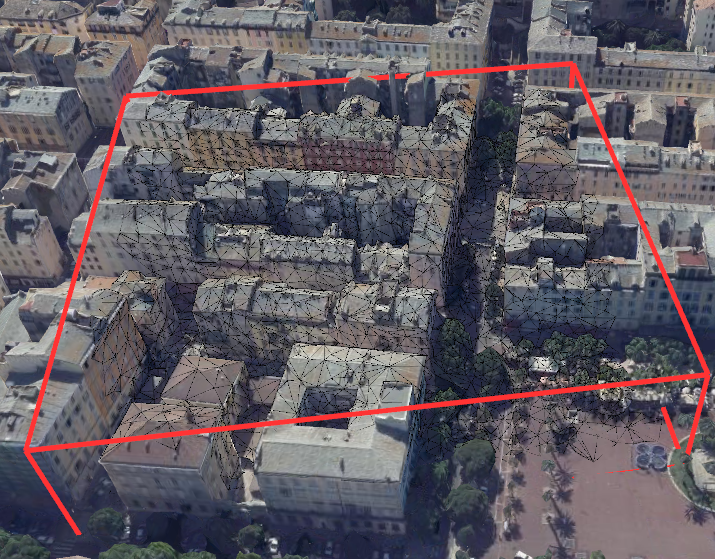
\includegraphics[width=0.65\textwidth]{images/Results/lod17_mesh.png}
    \caption{Bastia segment for elevation image strategy}
    \label{fig:bastia_mesh}
\end{figure}

\begin{figure}[H]
    \centering
    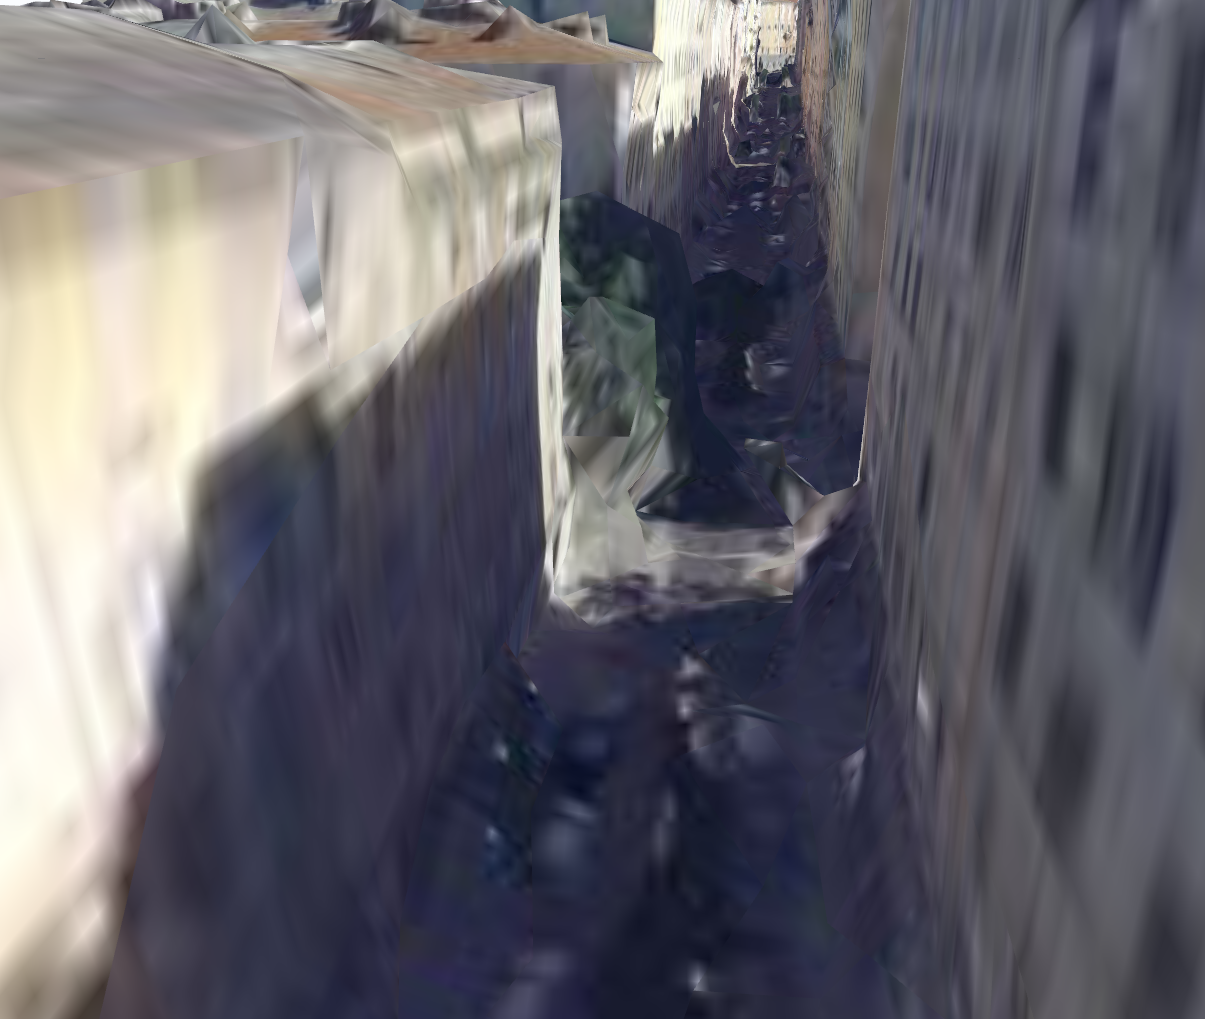
\includegraphics[width=0.65\textwidth]{images/Results/bastia_side_view.png}
    \caption{Side view of a street from Bastia dataset}
    \label{fig:Bastia_side_view}
\end{figure}

\subsection{Vertices interpolation for elevation images}
Fig.~\ref{fig:vertices_generation} illustrates the effects of interpolating more vertices for an elevation image approach. In a mesh representation, the vertices distribution is much sparser than in point clouds and the resulting elevation image is not usable. However, vertices interpolation leads to a satisfying elevation image, where it is clearly possible to distinguish objects outline. 
\begin{figure}[H]
        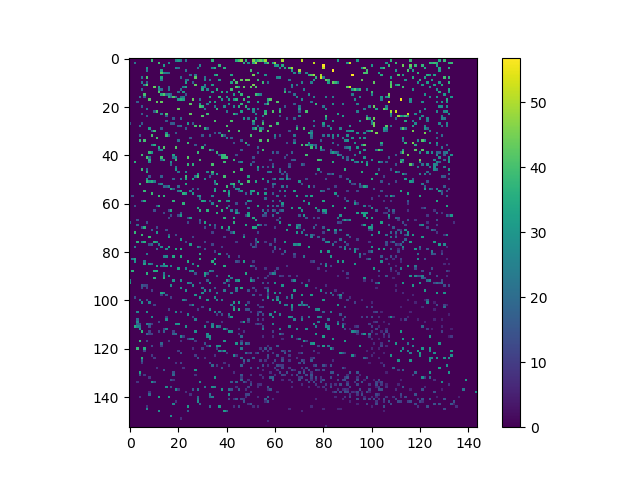
\includegraphics[width=0.5\textwidth]{images/Results/minimal_vertices.png} ~ 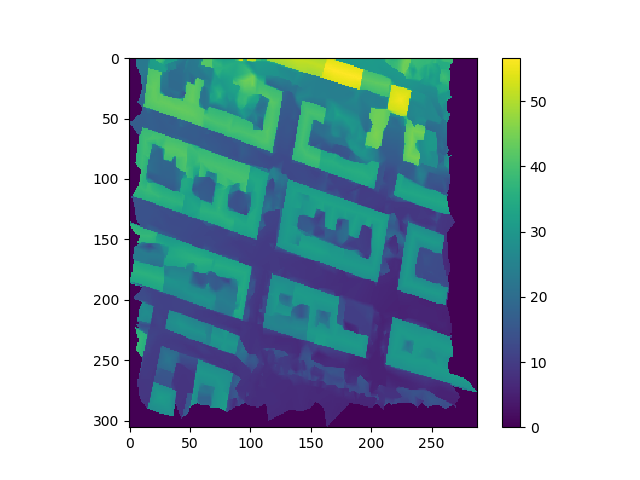
\includegraphics[width=0.5\textwidth]{images/Results/minimal_z_1msquare.png}
    
    \caption{Vertices interpolation for minimal elevation images}
    \label{fig:vertices_generation}
\end{figure}
Although such a method does not make up for the fact that the ground is not always represented, especially under wide objects such as trees, it seems promising enough to infer ground location as opposed to buildings location.

\subsection{Ground model generation}
As presented in the Methods chapter, two strategies were considered for obtaining a ground model from the elevation image. 
\subsubsection{Using $\lambda-$flat zone algorithm}
The results of the $\lambda-$flat zone algorithm for $\lambda = 0.5$ are represented in Fig.~\ref{fig:minimaAndGroundModel}.a, consisting in many segments due to the lack of continuity of the ground in the mesh representation. Fig.~\ref{fig:minimaAndGroundModel}.c represents the final ground model obtained by selecting only 0.5m-quasi flat zones containing a local minimum of the elevation image (Fig.~\ref{fig:minimaAndGroundModel}.b). This approach is very promising for high-resolution datasets. The irregularities around the buildings outline come from the presence of cars parked on the side of the street (as for instance in Fig.~\ref{fig:Bastia_side_view}). \\
However, in the case of Bastia dataset, areas that should be flat are sometimes captured as bumps and finding the perfect $\lambda$ gets complicated as it becomes almost impossible to discriminate between bumps corresponding to the road and other objects such as cars. 
\begin{figure}[H]
 \centering
        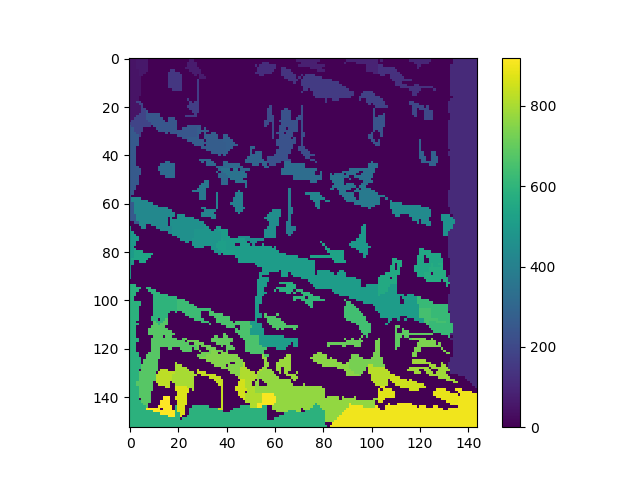
\includegraphics[width=0.45\textwidth]{images/Results/biggest_lambda_zones.png} ~ 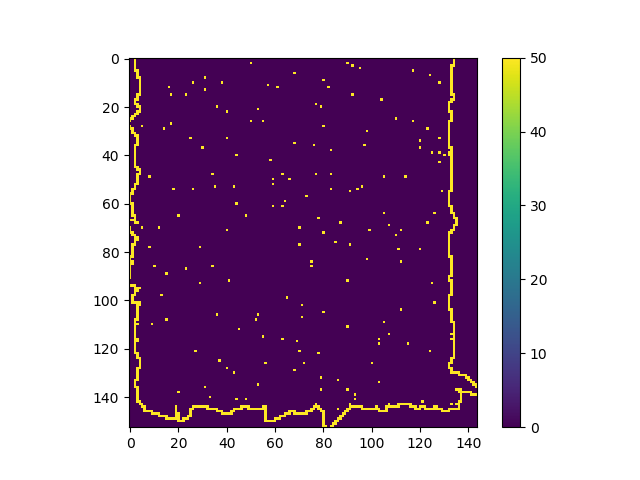
\includegraphics[width=0.45\textwidth]{images/Results/local_minima.png}  \\
      (a) Local minima \qquad  \qquad \qquad(b) $\lambda-$zones \\
   
    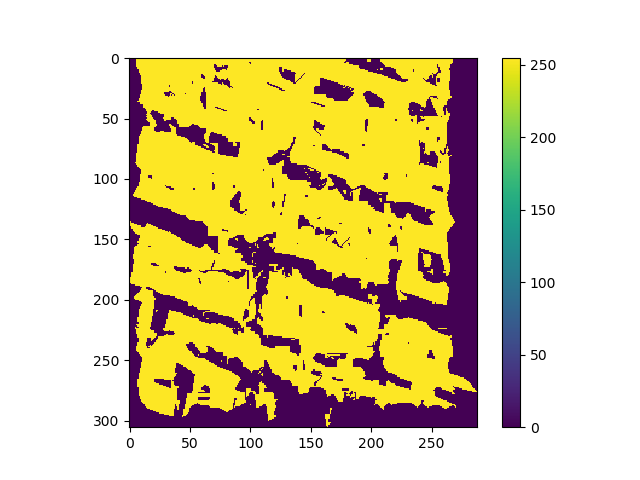
\includegraphics[width=0.7\textwidth]{images/Results/1msquare_zones.png}\\
    (c) Resulting ground model for $\lambda$=0.5m (ground in purple)
    
    \caption{$\lambda-$zone algorithm based ground detection}
    \label{fig:minimaAndGroundModel}
\end{figure}
\subsubsection{Using k-means clustering}
The ground model is depicted in Fig.~\ref{fig:k-means_gm}. The result approaches the intuition of the result, with the model indicating the zones where the objects we want to detect and identify will be located. It however struggles in the top right corner that corresponds to a steep slop into a court yard with high trees surrounded by buildings. 
\begin{figure}[H]
    \centering
    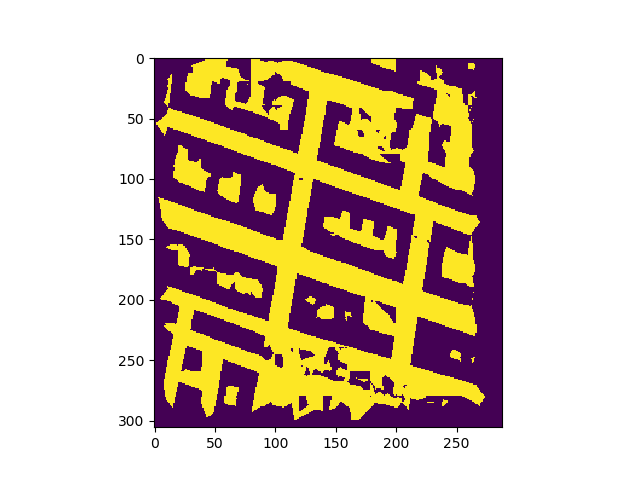
\includegraphics[width=0.8\textwidth]{images/Results/binary_ground.png}
    \caption{Ground model (yellow) using k-means clustering on the vertices}
    \label{fig:k-means_gm}
\end{figure}
\subsection{Backprojection}
The backprojection, represented on Fig.~\ref{fig:backproj}, is carried out on triangles projected onto the ground mask. However, using only verticality and elevation as clustering criteria, the façades are clustered but also some vertical triangles with the ground section. 
\begin{figure}[H]
    \centering
    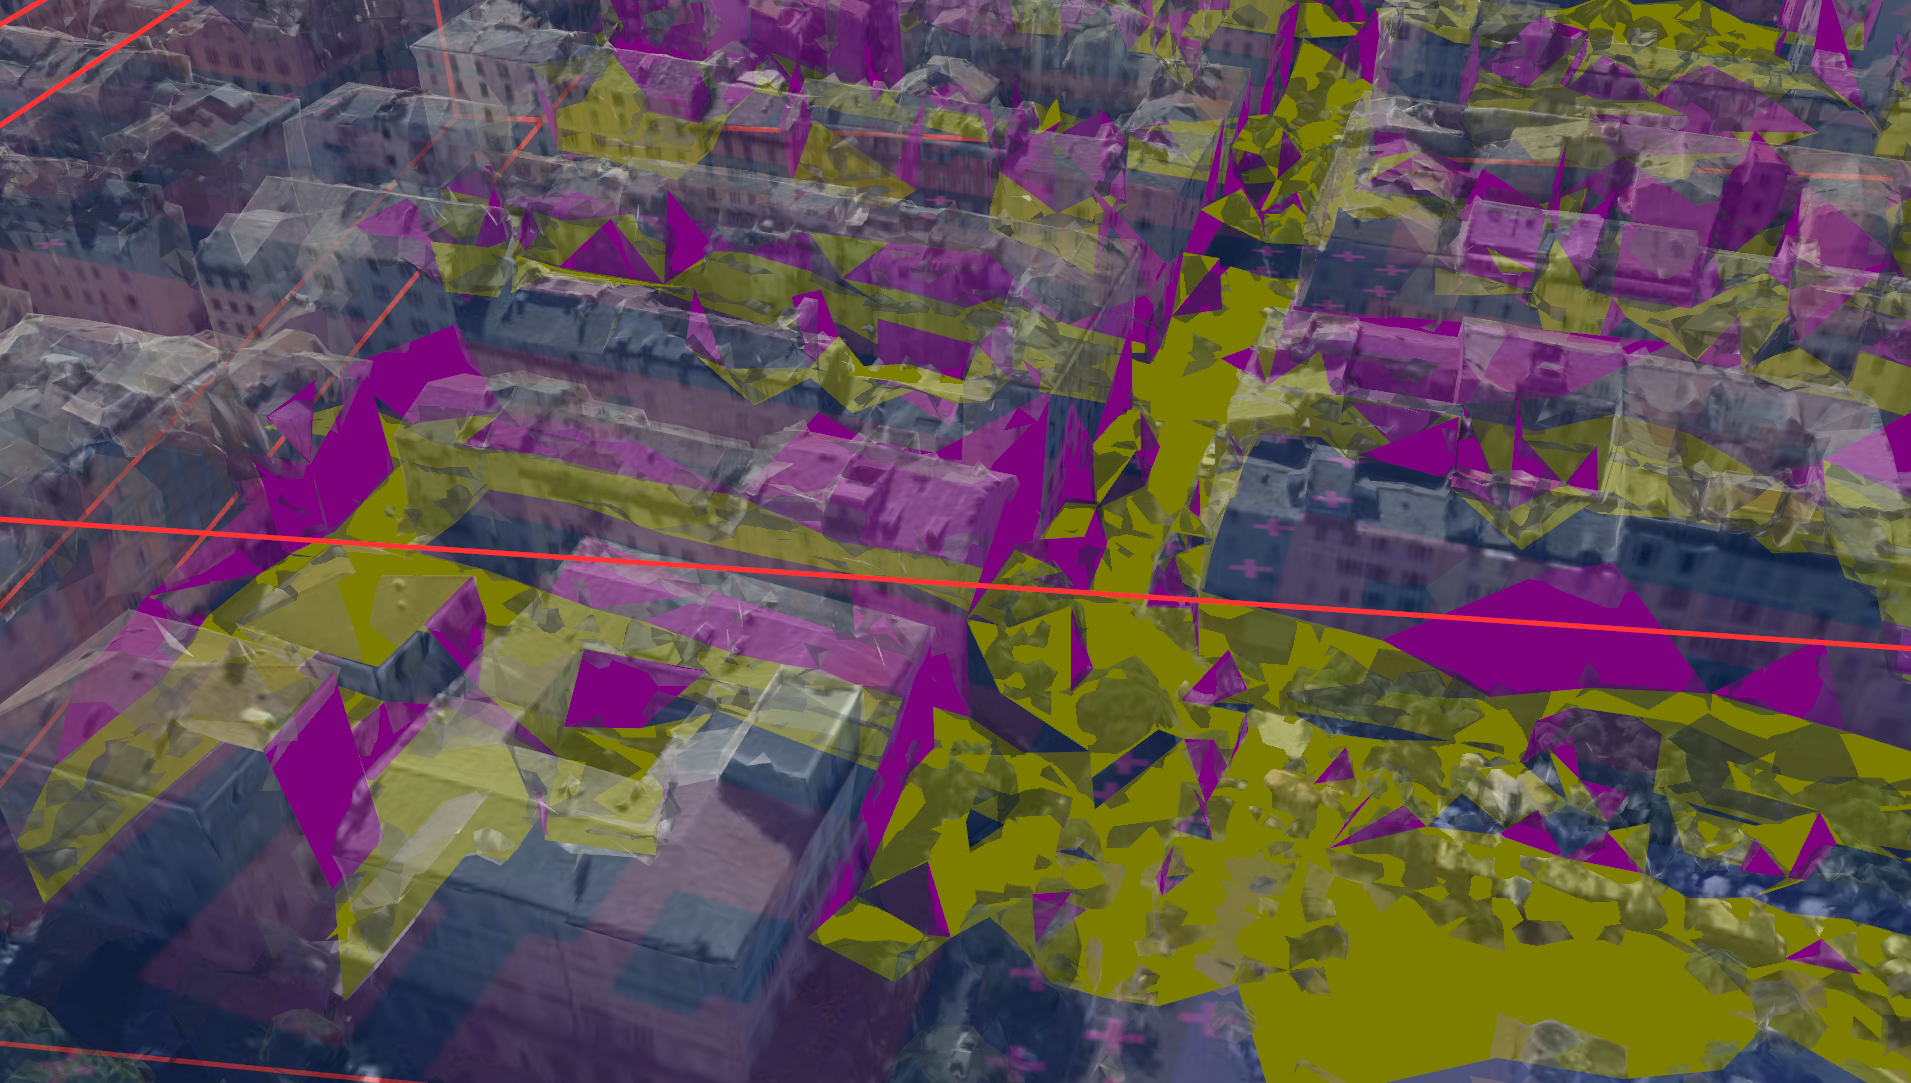
\includegraphics[width=0.8\textwidth]{images/Results/3D_triangles_ground.png}
    \caption{Backprojection of triangles belonging to the groundmodel}
    \label{fig:backproj}
\end{figure}
\subsection{Conclusion}
Although efficient on high-resolution meshes with rather low terrain elevation changes, the use of the $\lambda-$algorithm strategy is rather greedy in terms of computations and suffers on lower-resolution meshes. Performing clustering on interpolated vertices yields rather satisfying results, offering robustness to variability in a mesh resolution. However, when adopting such a strategy, the backprojection represents a challenge. \\
Overall, this approach is worth investigating and represents a historical step in this degree project. However, when faced with performing clustering on triangle properties for backprojection, the logical following step was to investigate direct clustering of the triangles. 

\section{Feature extraction}
Feature extraction is a critical step in mesh segmentation, especially more so for an unsupervised approach, such as the one used in this project. The features need to be able to describe and discriminate different objects. Although geometrical features such as elevation and horizontality perform very well for structures such as roofs and façades in flat urban environments, complications arise as smaller structures are captured on roads and the ground slope gets steeper.
\subsection{Elevation} 
Elevation is a rather straight-forward feature but the choice of the window size is critical to adapt to buildings in hilly environments and large flat terrains. Needless to say that a unique window size is most of the time not sufficient. \\
Fig~\ref{fig:elev_Helsinki} shows the elevation feature of each triangle with a window size of 50m (which means an rectangular area of 50m x 50m around the triangle). This window size is not enough to accommodate for very large flat areas such as the middle square where slight changes in height lead to high variations of the elevation features. It can also be noticed that lower structures close to very high buildings will have lower elevation scores as well. 

\begin{figure}[H]
    \centering
    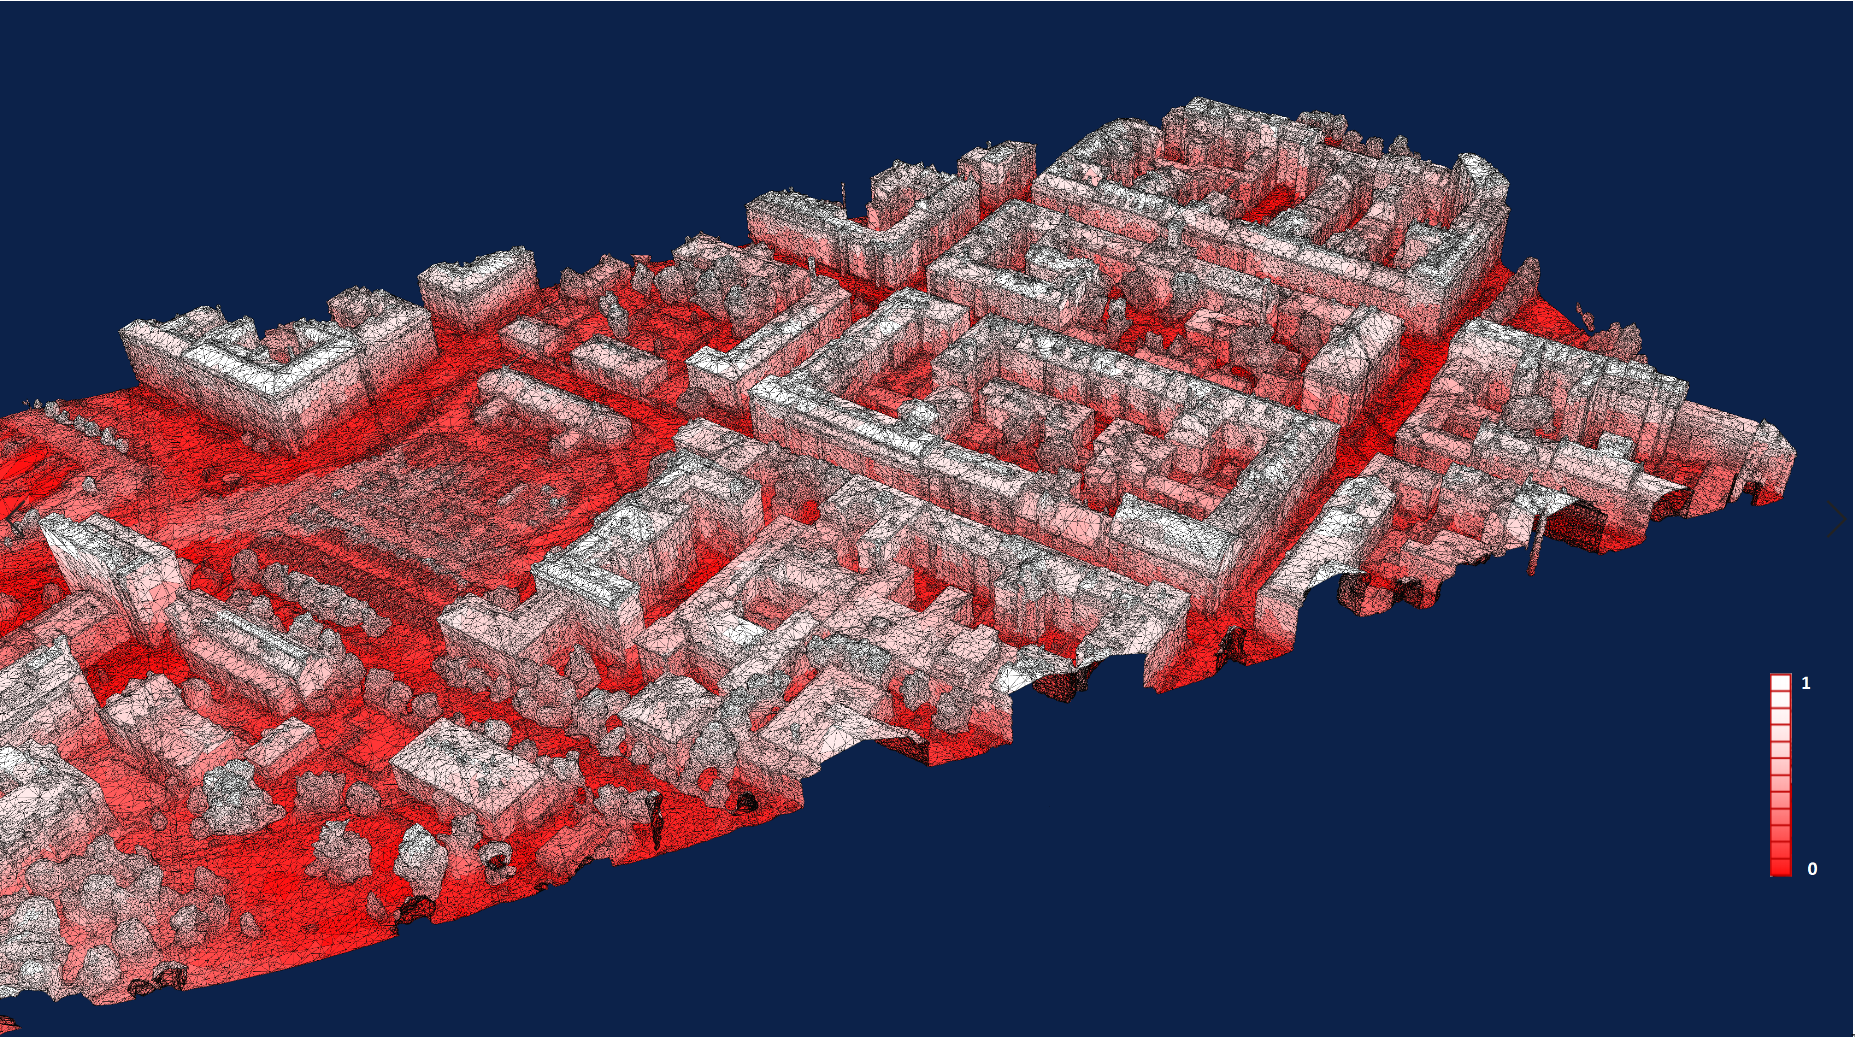
\includegraphics[width=0.9\textwidth]{images/features/elevation_50_Helsinki.png}
    \caption{Elevation feature on Helsinki data using a window of 50m}
    \label{fig:elev_Helsinki}
\end{figure}
\subsection{Horizontality}
Of all the features presented in this project, the horizontality feature is probably the most straight-forward and the easiest to compute, as it does not require any user-input parameters or approximations. Presented on a segment of Bastia (Fig.~\ref{fig:bastia_density}), the horizontality value of the triangles is visualised on Fig.~\ref{fig:bastia_horizontality}. It appears to be very efficient for the clustering of very geometrically shaped structures such as buildings. 


\begin{figure}[H]
    \centering
    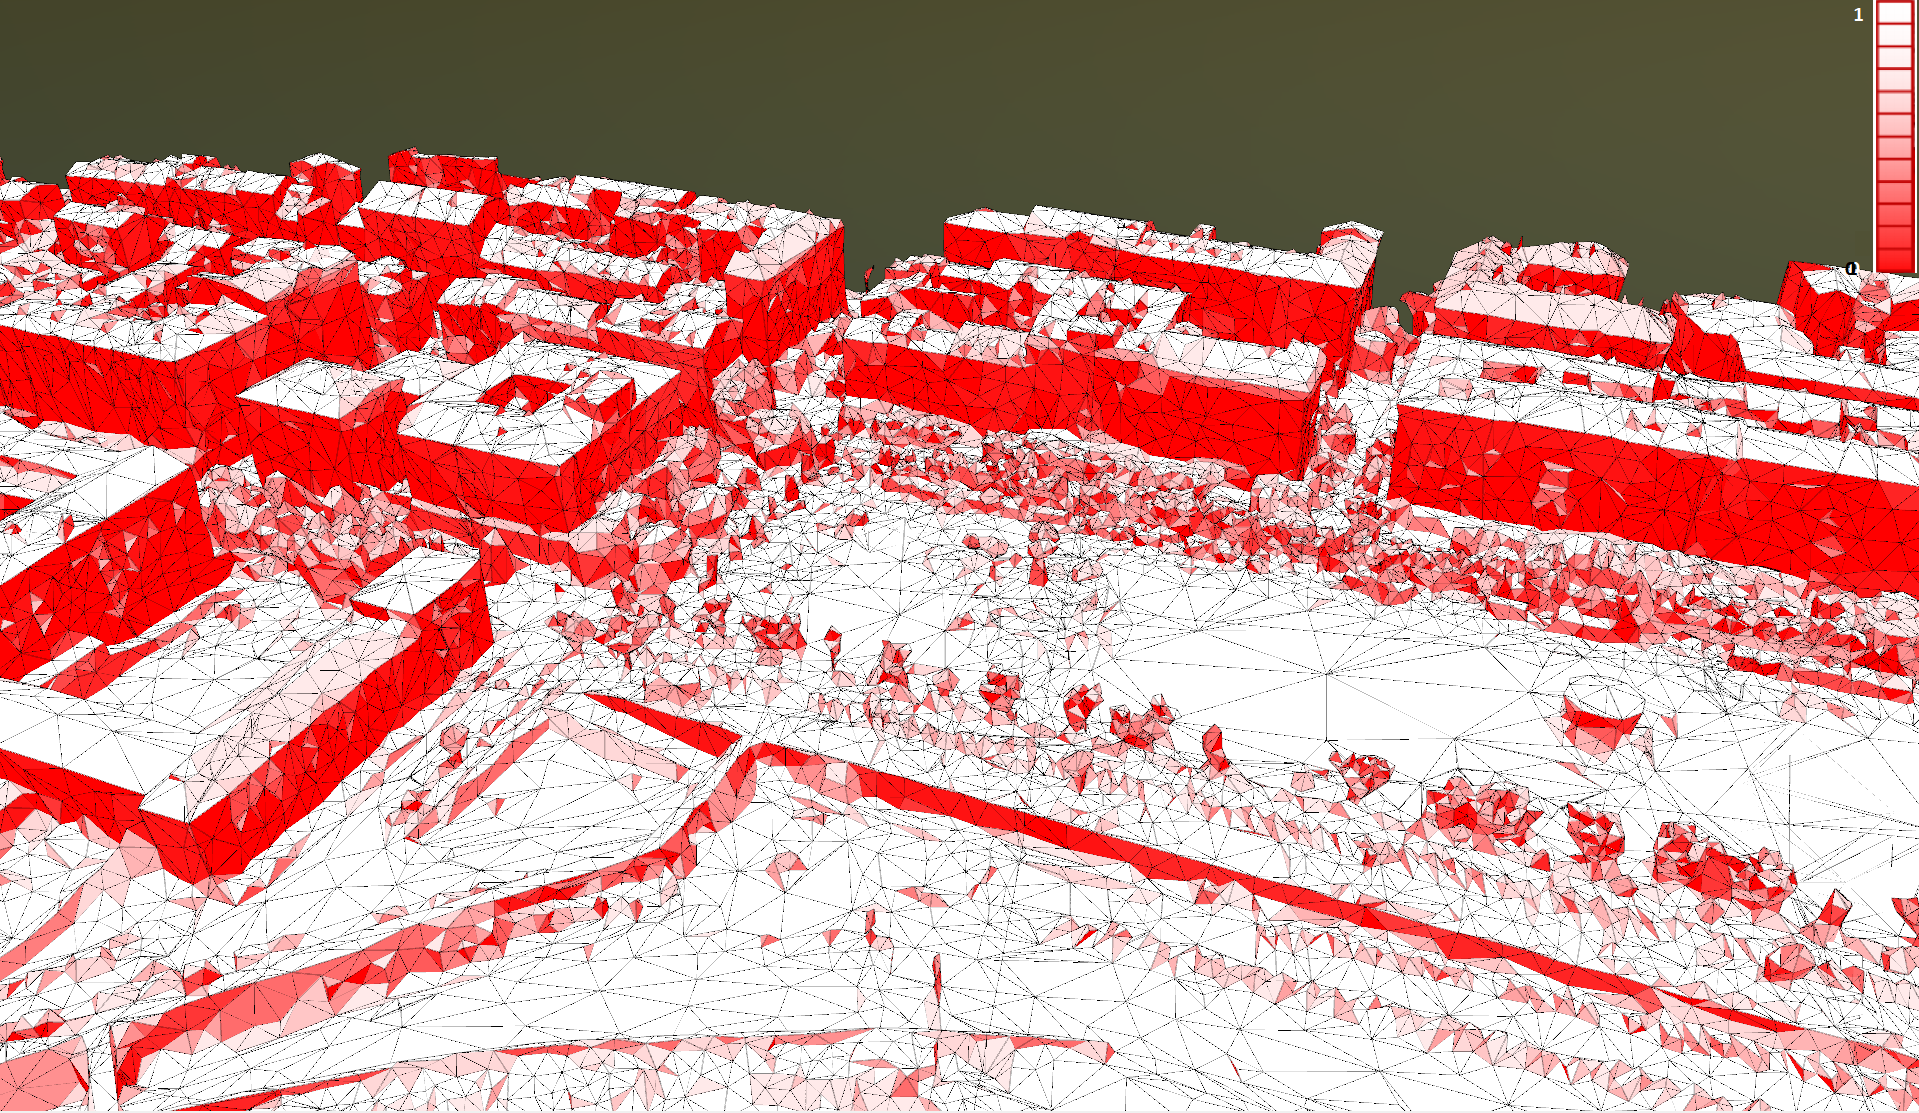
\includegraphics[width=0.9\textwidth]{images/features/horizontality_bastia.png}
    \caption{Horizontality feature visualisation on Bastia dataset}
    \label{fig:bastia_horizontality}
\end{figure}

\subsection{Planarity}
Planarity is a more problematic feature. It is represented on Fig.~\ref{fig:bastia_planarity}, on the same segment of Bastia mesh as previously (Fig.~\ref{fig:bastia_density}). In ideal cases or high-resolution models, buildings and grounds would score high while irregular objects such as trees would score low. However, as in the case of Bastia dataset, the reconstruction quality leads to bumps in place of flat areas, therefore leading to lower-scoring for areas that were initially planar. 
\begin{figure}[H]
    \centering
    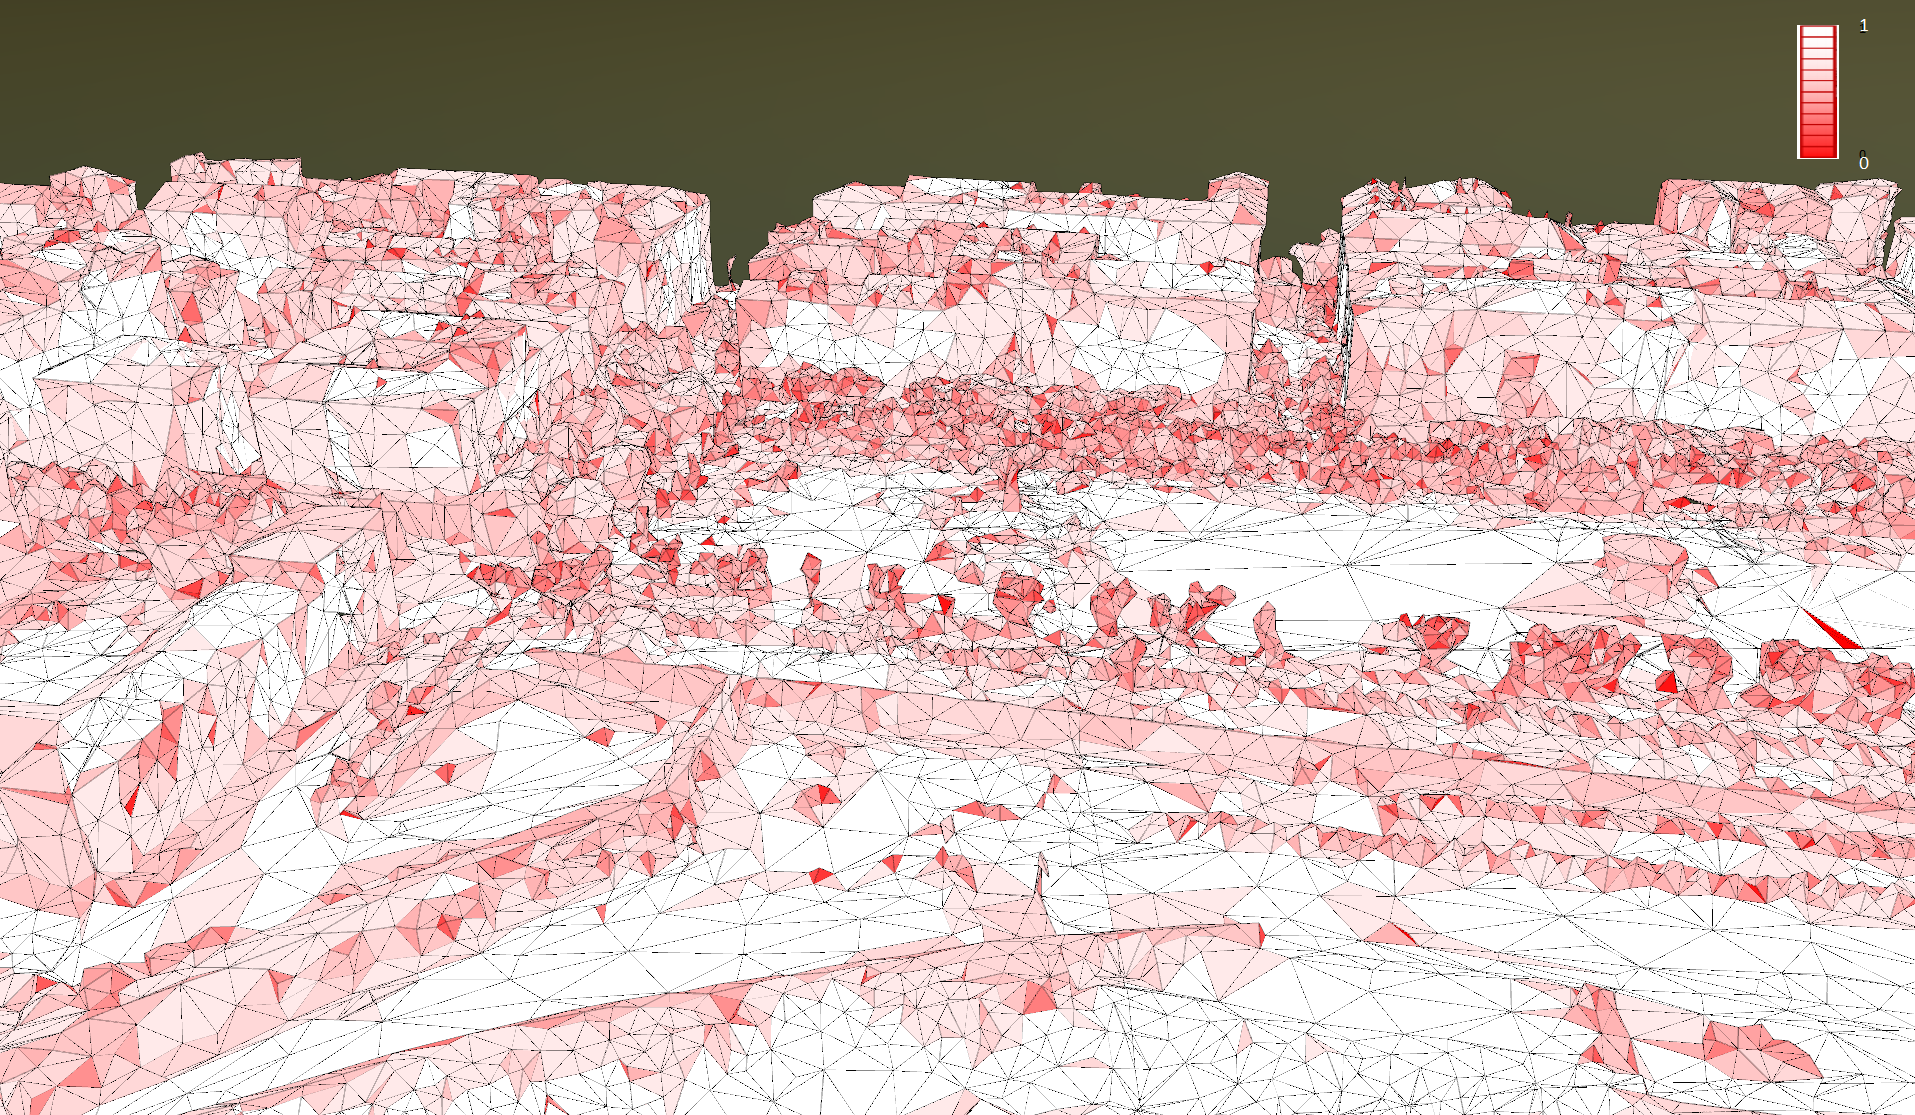
\includegraphics[width=\textwidth]{images/features/planarity_bastia.png}
    \caption{Planarity feature visualisation on Bastia dataset}
    \label{fig:bastia_planarity}
\end{figure}
\subsection{Greenness}
The greenness feature was forgotten rather fast when exploring relevant features for trees detection. One of the main reasons, that can be observed on Fig.~\ref{fig:greenness_text} and Fig.~\ref{fig:greenness_closeup}, is that although the overall colour of the texture mapping of trees triangles is green, it contains a lot of black pixels whose hue value is not green and therefore the average HSV colour value of the triangle would not score high in terms of greenness even though it contains green. \\

\begin{figure}[H]
    \centering
    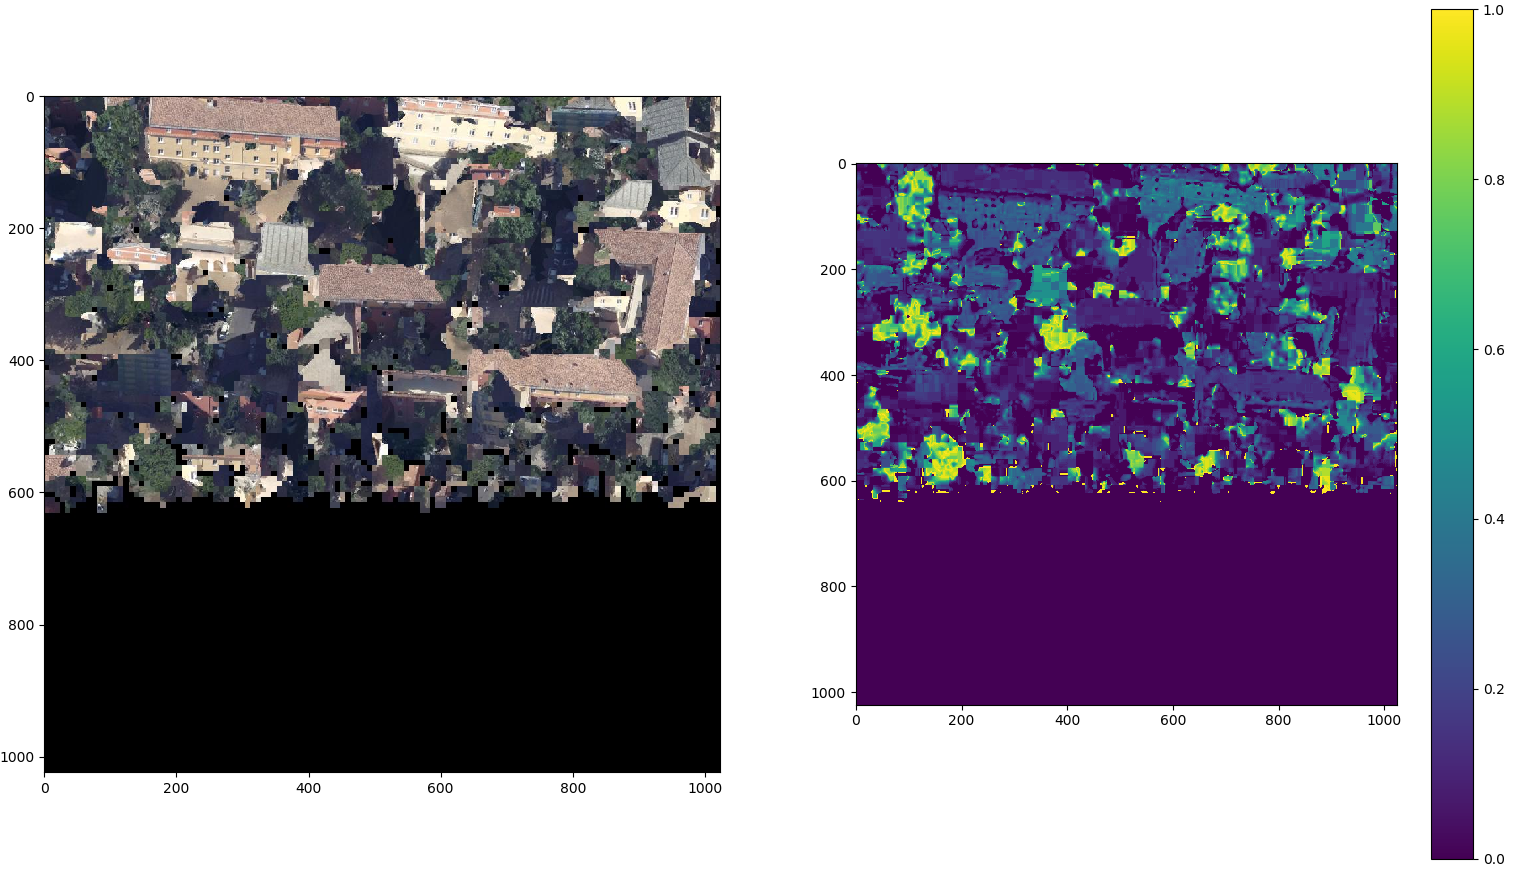
\includegraphics[width=\textwidth]{images/features/greenness_texture.png}
    \caption{Texture from Bastia dataset and associated pixel-wise greenness}
    \label{fig:greenness_text}
\end{figure}
\begin{figure}[H]
    \centering
    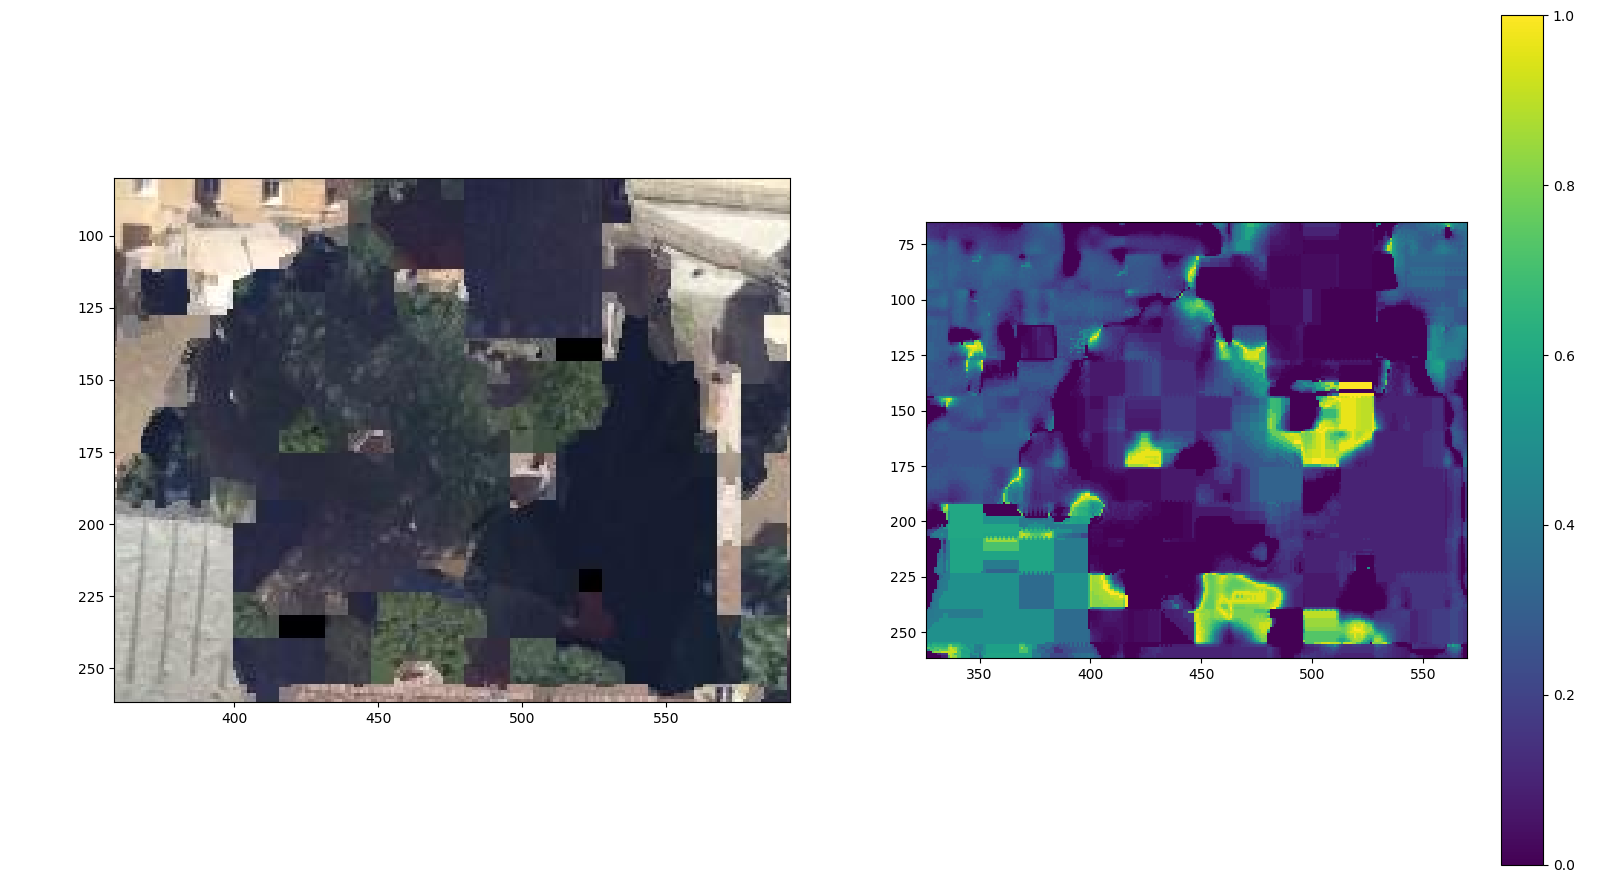
\includegraphics[width=\textwidth]{images/features/greenness_closeup.png}
    \caption{Zoom-up on a portion of Fig.~\ref{fig:greenness_text}}
    \label{fig:greenness_closeup}
\end{figure}
\subsection{Density}
The density feature feature seems very promising.  Computed from the vertices count on 1m x 1m windows, the resulting image was smoothed using an average filter with kernel of size 10x10 before computing the density feature value as presented in the Methods section. \\
Bastia and Helsinki datasets present different resolutions, with Bastia dataset having a lower-resolution leading to many bumps in flat areas and poorly reconstructed trees while Helsinki dataset has a higher resolution, with more triangles for objects representation. Fig.~\ref{fig:hels_density} and Fig.~\ref{fig:bastia_density} represent the density value for 1m x 1m areas. On the picture, it is rather evident that trees and façades mark the density map with high scores while grounds and roofs score lower values. On Helsinki dataset, smaller objects such as cars parked in a square can also be recognised from the pictures, opening to the possibility of using it for objects detection within the mesh as well. 
\begin{figure}[H]
    \centering
    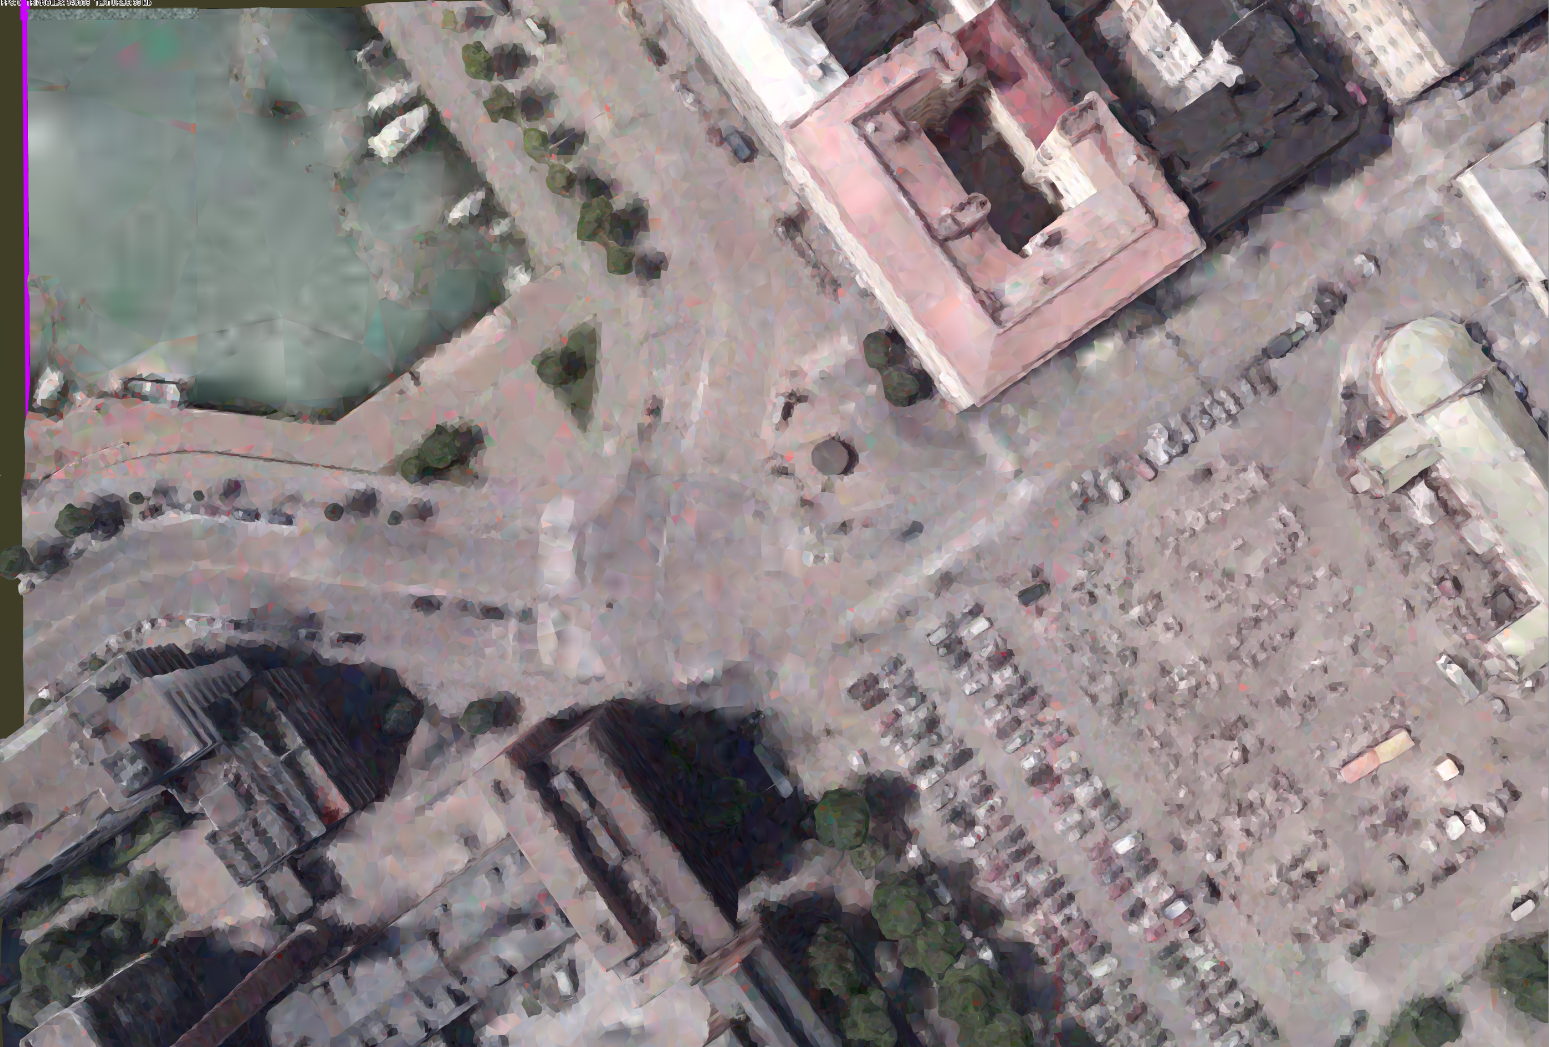
\includegraphics[width=0.40\textwidth]{images/features/helsinki_tree.png} ~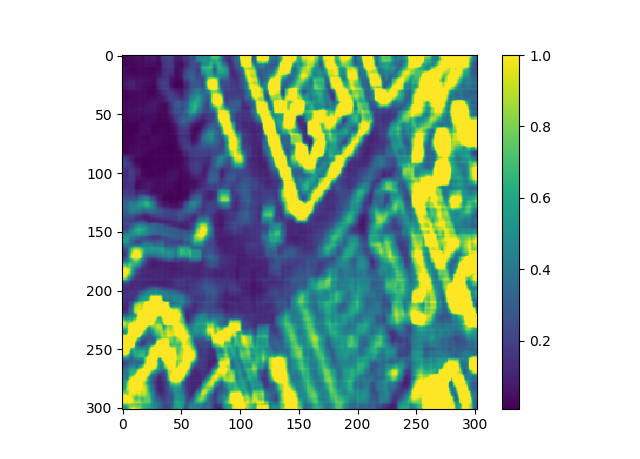
\includegraphics[width=0.55\textwidth]{images/features/density_helsinki_tree.png}
    \caption{Density feature evaluation on Helsinki dataset}
    \label{fig:hels_density}
\end{figure}
\begin{figure}[H]
    \centering
    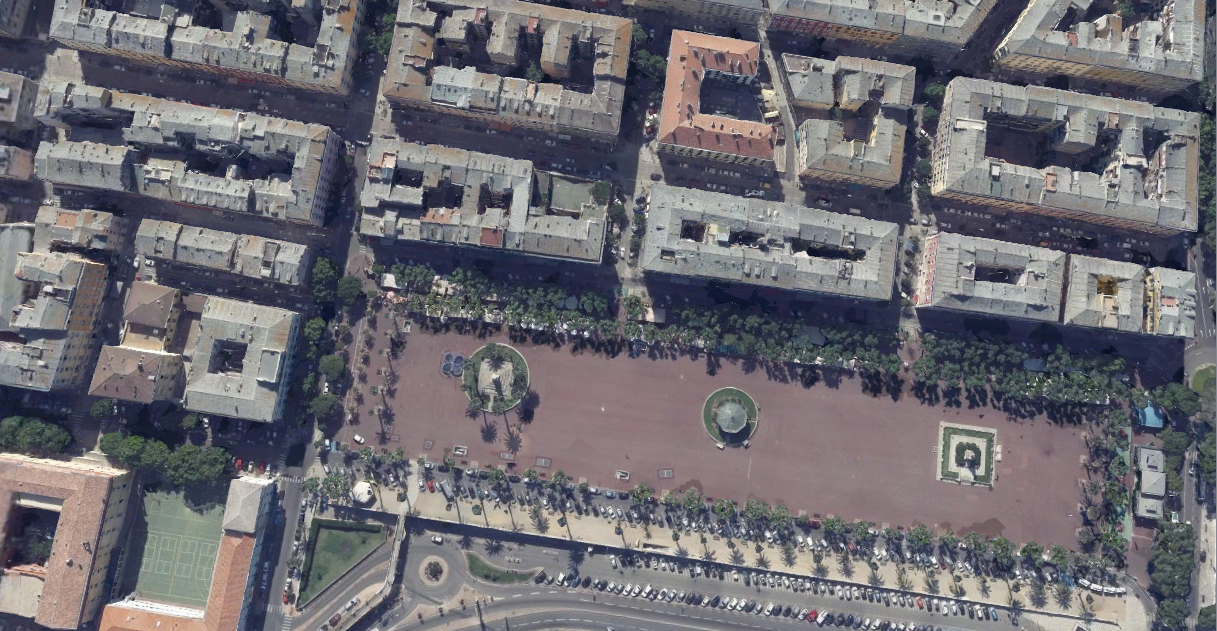
\includegraphics[width=0.38\textwidth]{images/features/bastia_view.png} ~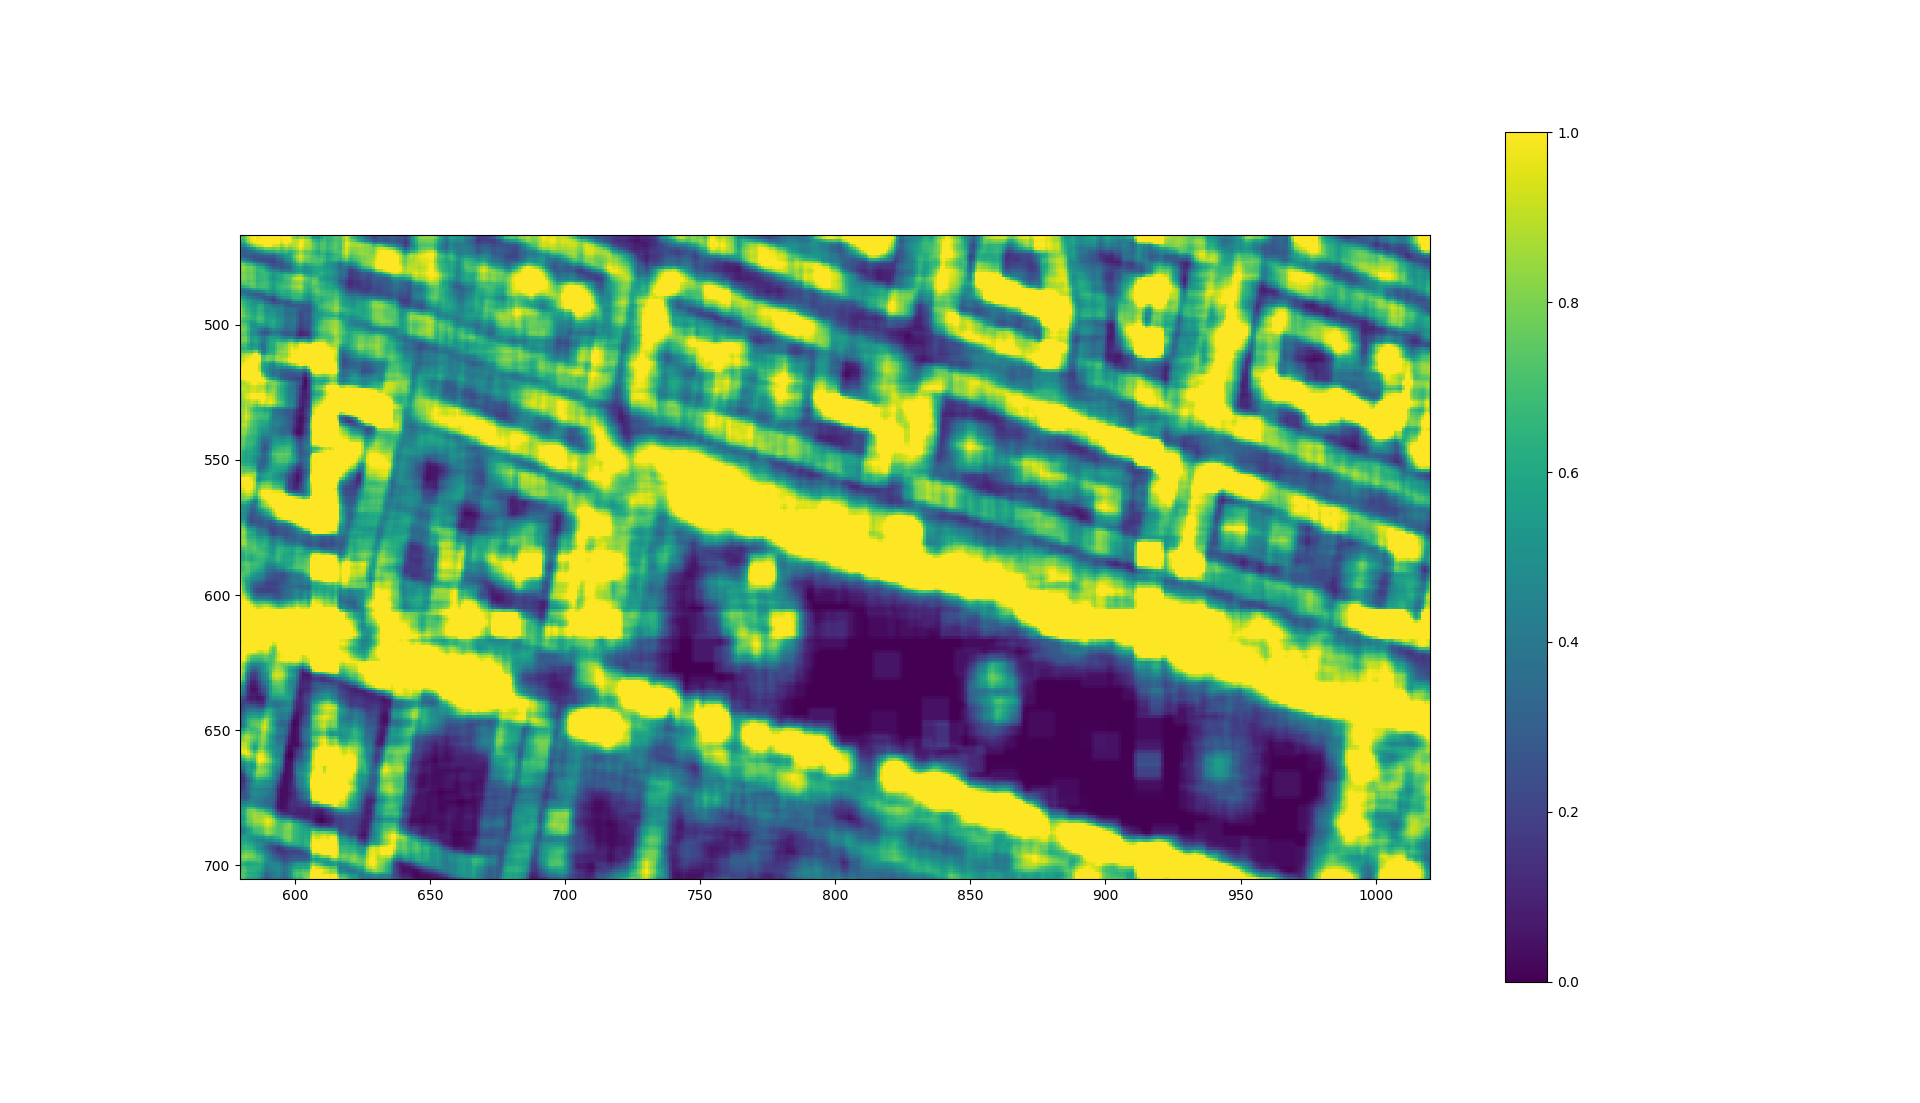
\includegraphics[width=0.60\textwidth]{images/features/bastia_density_tree.png}
    \caption{Density feature evaluation on Bastia dataset}
    \label{fig:bastia_density}
\end{figure}

\subsection{Conclusion}
Features selection is critical for correct classification of triangles, in order to capture discriminative information. The set of features used in this work are mostly geometric and seem suitable to adapt to both higher- and lower-resolution meshes for artefact detection. 
\section{Artefacts detection algorithm}
This section presents the results for several steps of the algorithm as well general conclusions on the techniques used and their potential for artefact detection in lower-resolution meshes. 
\subsection{Connectivity analysis}
For finer resolution datasets such as Helsinki dataset, there are not any significant results while performing this analysis. However, when carried out on Bastia dataset, two main types of disconnected components were identified (Fig.~\ref{fig:bastia_connec_analysis_types_of_comp}). The first ones (Fig.~\ref{fig:bastia_connec_analysis_tree artefacts}), whose detection and identification can be interesting, tree artefacts, small bushes-like components either visually connected to the rest of the tree or simply flying above the location of the tree in the original data. The second ones correspond to manual fixes so that the data visually matches, such as the building corner segment seen on Fig.~\ref{fig:bastia_connec_analysis_types_of_comp}. \\
\begin{figure}[H]
    \centering
    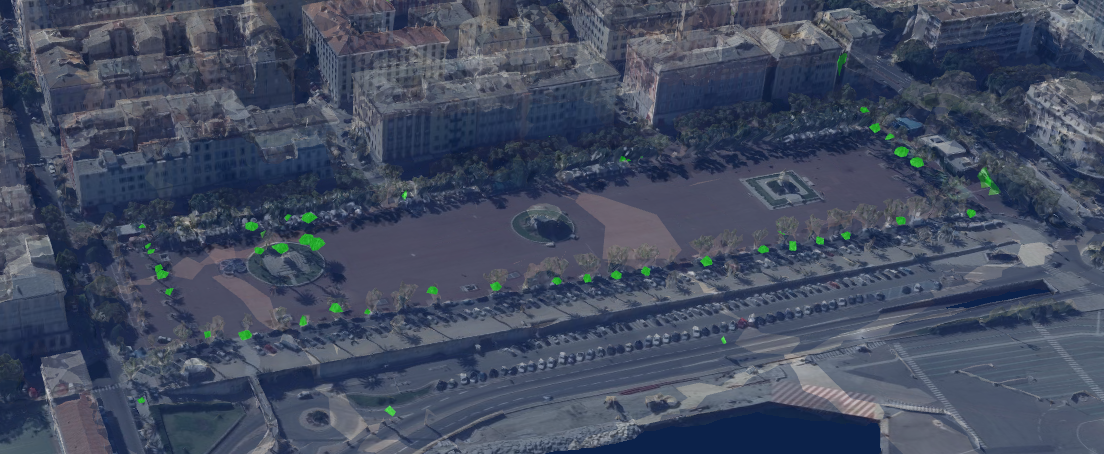
\includegraphics[width=0.45\textwidth]{images/Connectivity_Analysis/flying_bushes.png}
    \caption{Connectivity analysis in Bastia: tree artefacts (bright green) }
    \label{fig:bastia_connec_analysis_tree artefacts}
\end{figure}

\begin{figure}[H]
    \centering
    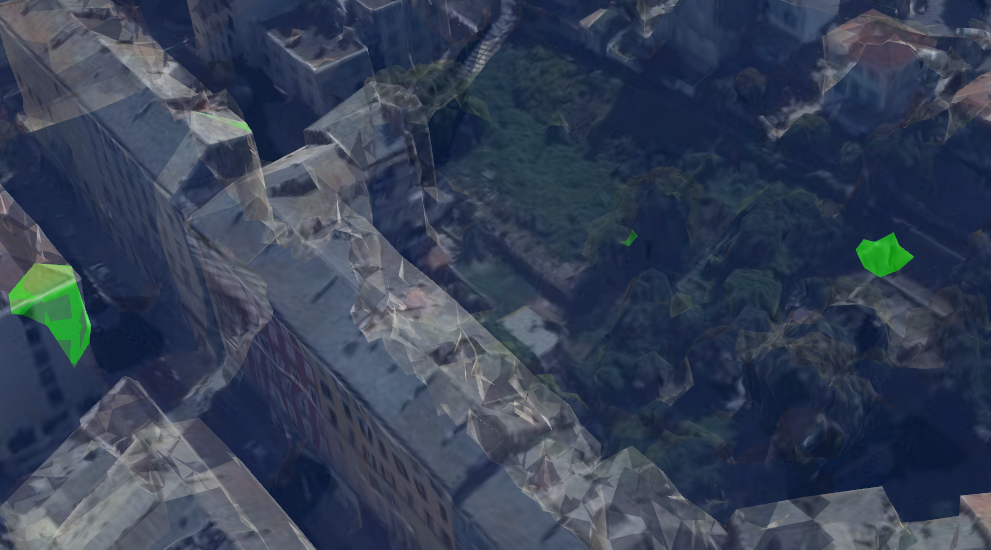
\includegraphics[width=0.45\textwidth]{images/Connectivity_Analysis/type_of_disc_objects.png}
    \caption{Connectivity analysis in Bastia: Two main types of disconnected components }
    \label{fig:bastia_connec_analysis_types_of_comp}
\end{figure}
Connectivity analysis results could be used to isolate objects and add them to the pool of objects to be classified in the last step of the algorithm. Additionally, the number of found disconnected components could be used as an indicator of the quality of a model reconstruction. 

\subsection{k-means}
The k-means approach represented a chronological step in the project timeline: this method is easier to apprehend and available in libraries. As the results (see Fig. ) were rather encouraging at first, the k-means approach helped put more weight and focus on feature extraction and serves as a control indicator as it provides information on the data being clustered. Additionally, k-means formulation allows to evaluate faster the influence and discriminating power of features without having to design unary terms. \\
Performed on Fig.~\ref{fig:bastia_mesh}, the results of the triangles clustering is presented in Fig.~\ref{fig:k-means_bastia}
\begin{figure}[H]
    \centering
    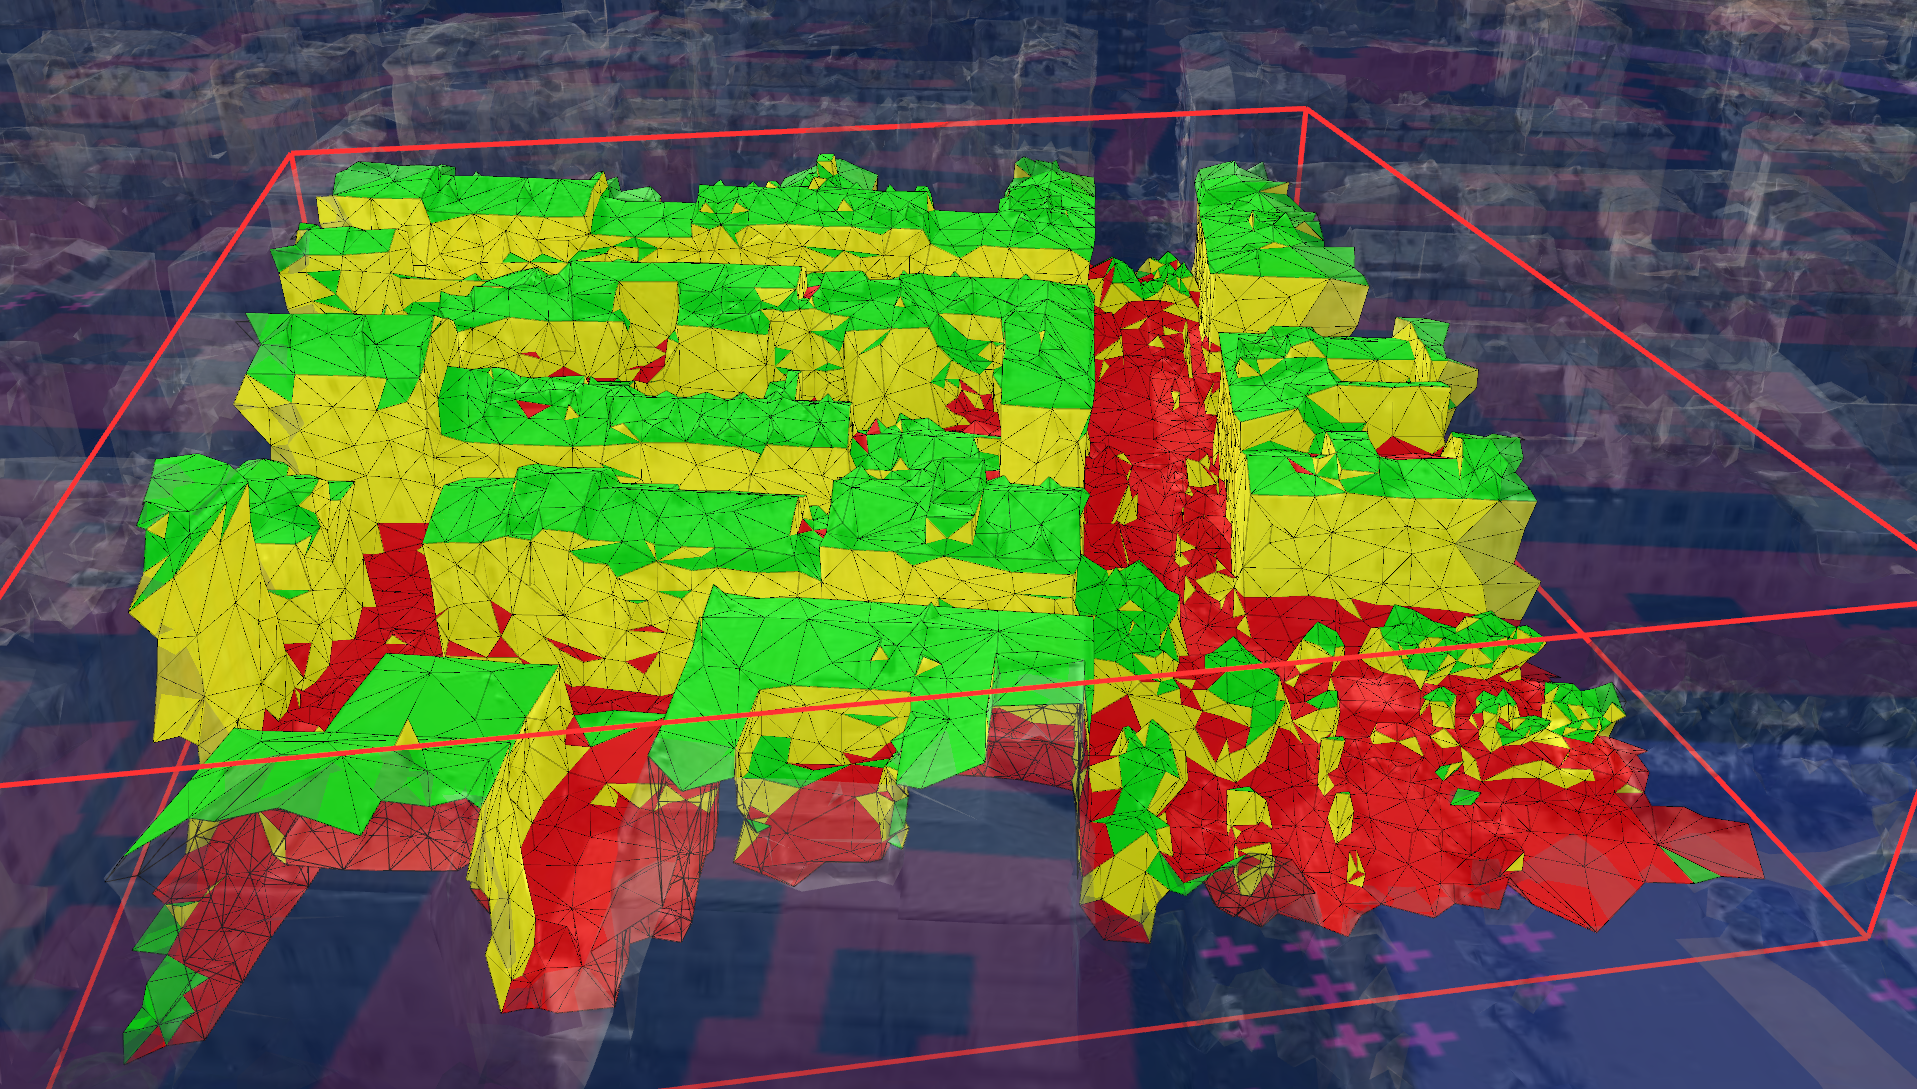
\includegraphics[width=0.45\textwidth]{images/Results/lod17_rouhani.png}~
    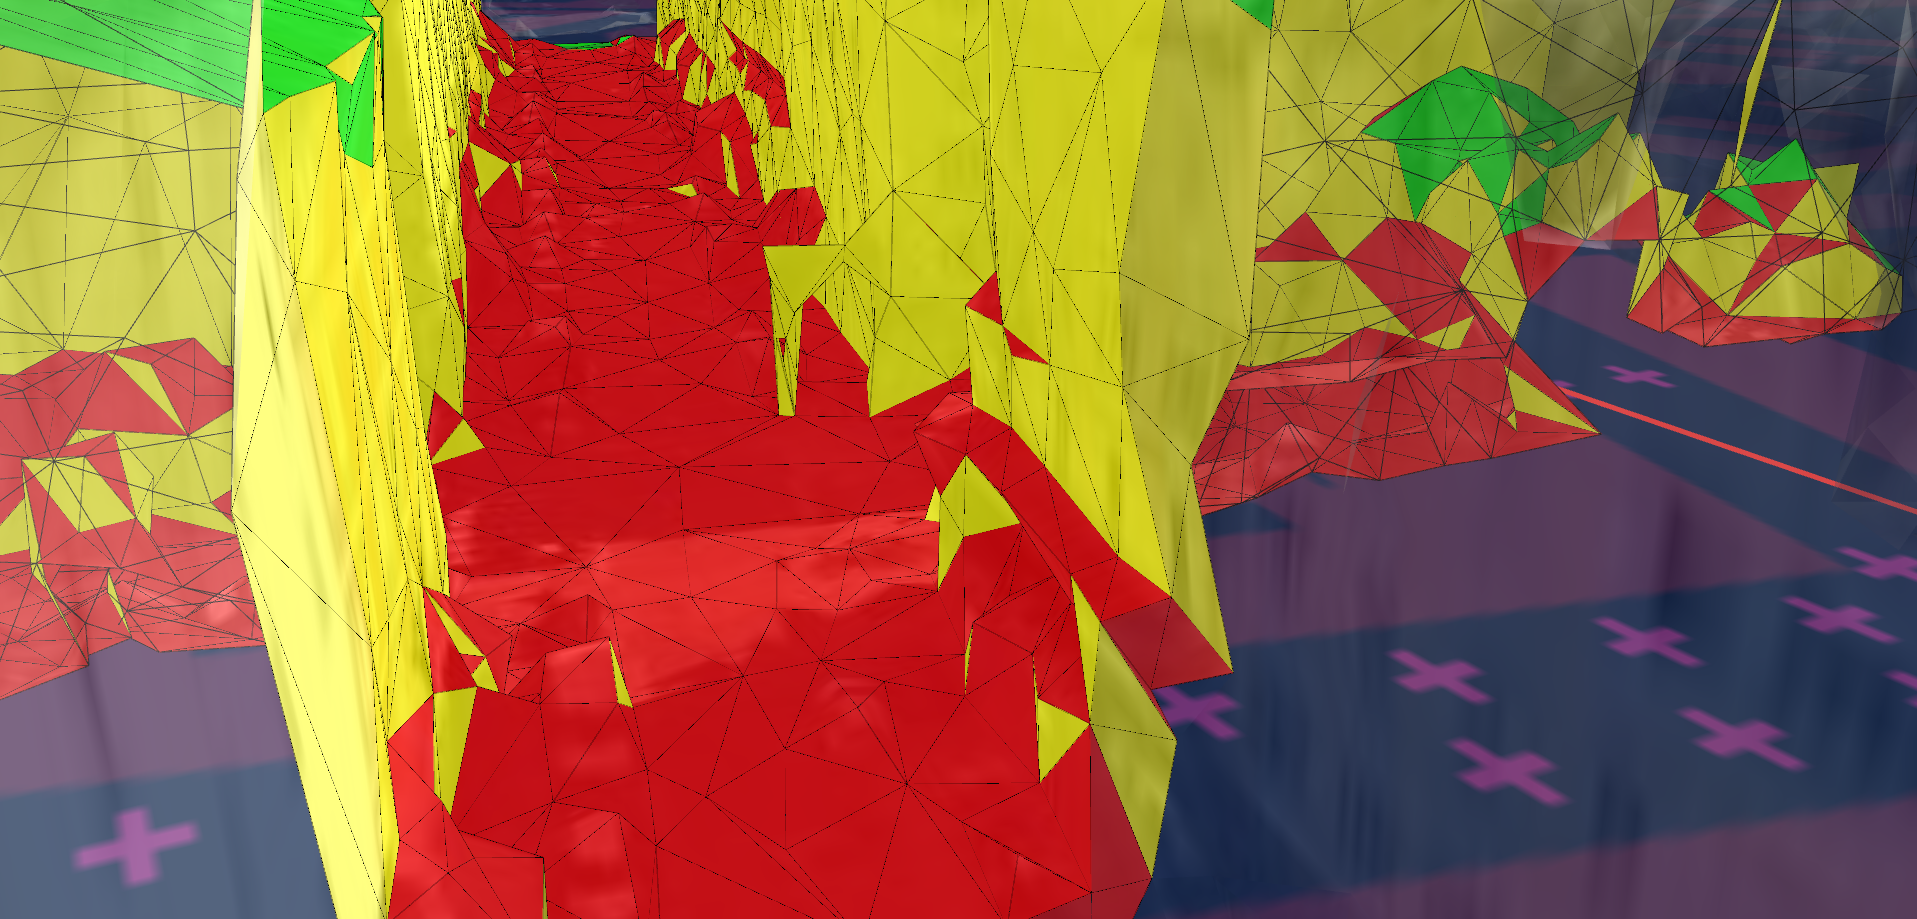
\includegraphics[width=0.45\textwidth]{images/Results/lod17_rouhani_otherview.png}
    \caption{k-means clustering on Bastia dataset}
    \label{fig:k-means_bastia}
\end{figure}
\subsection{Postprocessing rules}
First designed for k-means as a way to include contextual information, they were kept even with the MRF formulation as they help pally minor misclassifications. Postprocessing rules were applied on Fig.~\ref{fig:k-means_bastia} and the result is presented in Fig.~\ref{fig:bastia_postproc}.
\begin{figure}[H]
    \centering
    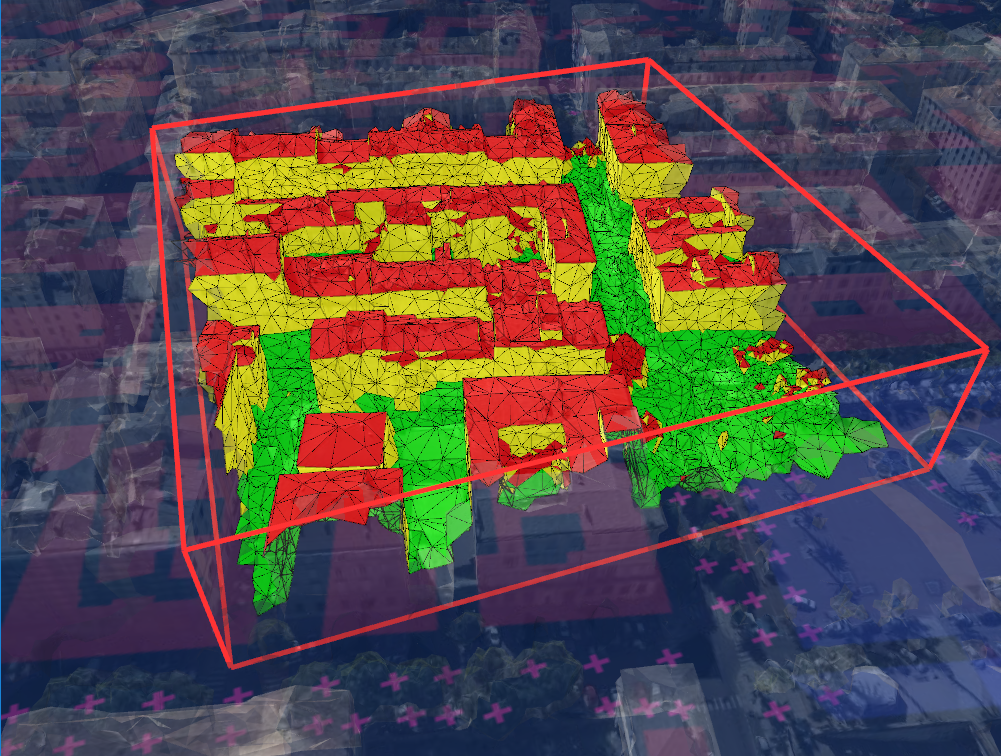
\includegraphics[width=0.9\textwidth]{images/Results/lod17_rouhani_additional_rules.png}
    \caption{Postprocessing rules on k-means clustering}
    \label{fig:bastia_postproc}
\end{figure}
\subsection{Superfacet clustering}
The urge for superfacets arose when the MRF formulation was chosen, as it significantly improved computation times without . However, due to the resolution of meshes and that triangles are in general larger in the datasets used in this work compared to those used in the literature: for instance, the 300mx300m  Paris mesh \textcite{rouhani} use contains around 1M triangular facets while a similar portion of the Paris dataset used in this work contains around 10 times less triangles, that is to say about 100k triangles. \\
Therefore, the superfacet clustering, otherwise less needed, used with a size threshold of 100m$^2$, a geometrical threshold of 30\degree and a photometric threshold of 60 in the colour space, performed in Paris has the following characteristics in terms of superfacets size (number of triangles) and area: $mean_{size}=2.15, variance_{size}=5.17, minmax_{size}=(1,22)$ and $mean_{area}=16.05, variance_{area}=635.88, minmax_{area}=(7.42e-05, 148.09)$. \\
Note that the maximal area exceeding the threshold comes from single triangles representing flat terrain. 
\subsection{MRF formulation}
The MRF formulation performs rather well according to an anticipated rationale. In this section, we show that the formulation used in \textcite{verdie} is not enough to accommodate to lower resolution meshes. In order to demonstrate this statement, the four-classes formulation was run onto a segment of Paris dataset, similar to the one used in the original paper. The results are shown in Fig.~\ref{fig:paris_verdie_mrf4}. On Fig.\ref{fig:paris_verdie_mrf3}, a similar formulation is used, removing the vegetation class. \\
The latter formulation yields rather satisfying results across the different datasets, with in general the same problems and misclassification as in the other papers: vegetation misclassified as partial roof and façade, large flat areas having parts misclassified as façade and buildings. The buildings detection with this formulation still holds and allows to generate a ground mesh from which objects can be segmented. 

\begin{figure}[H]
    \centering
    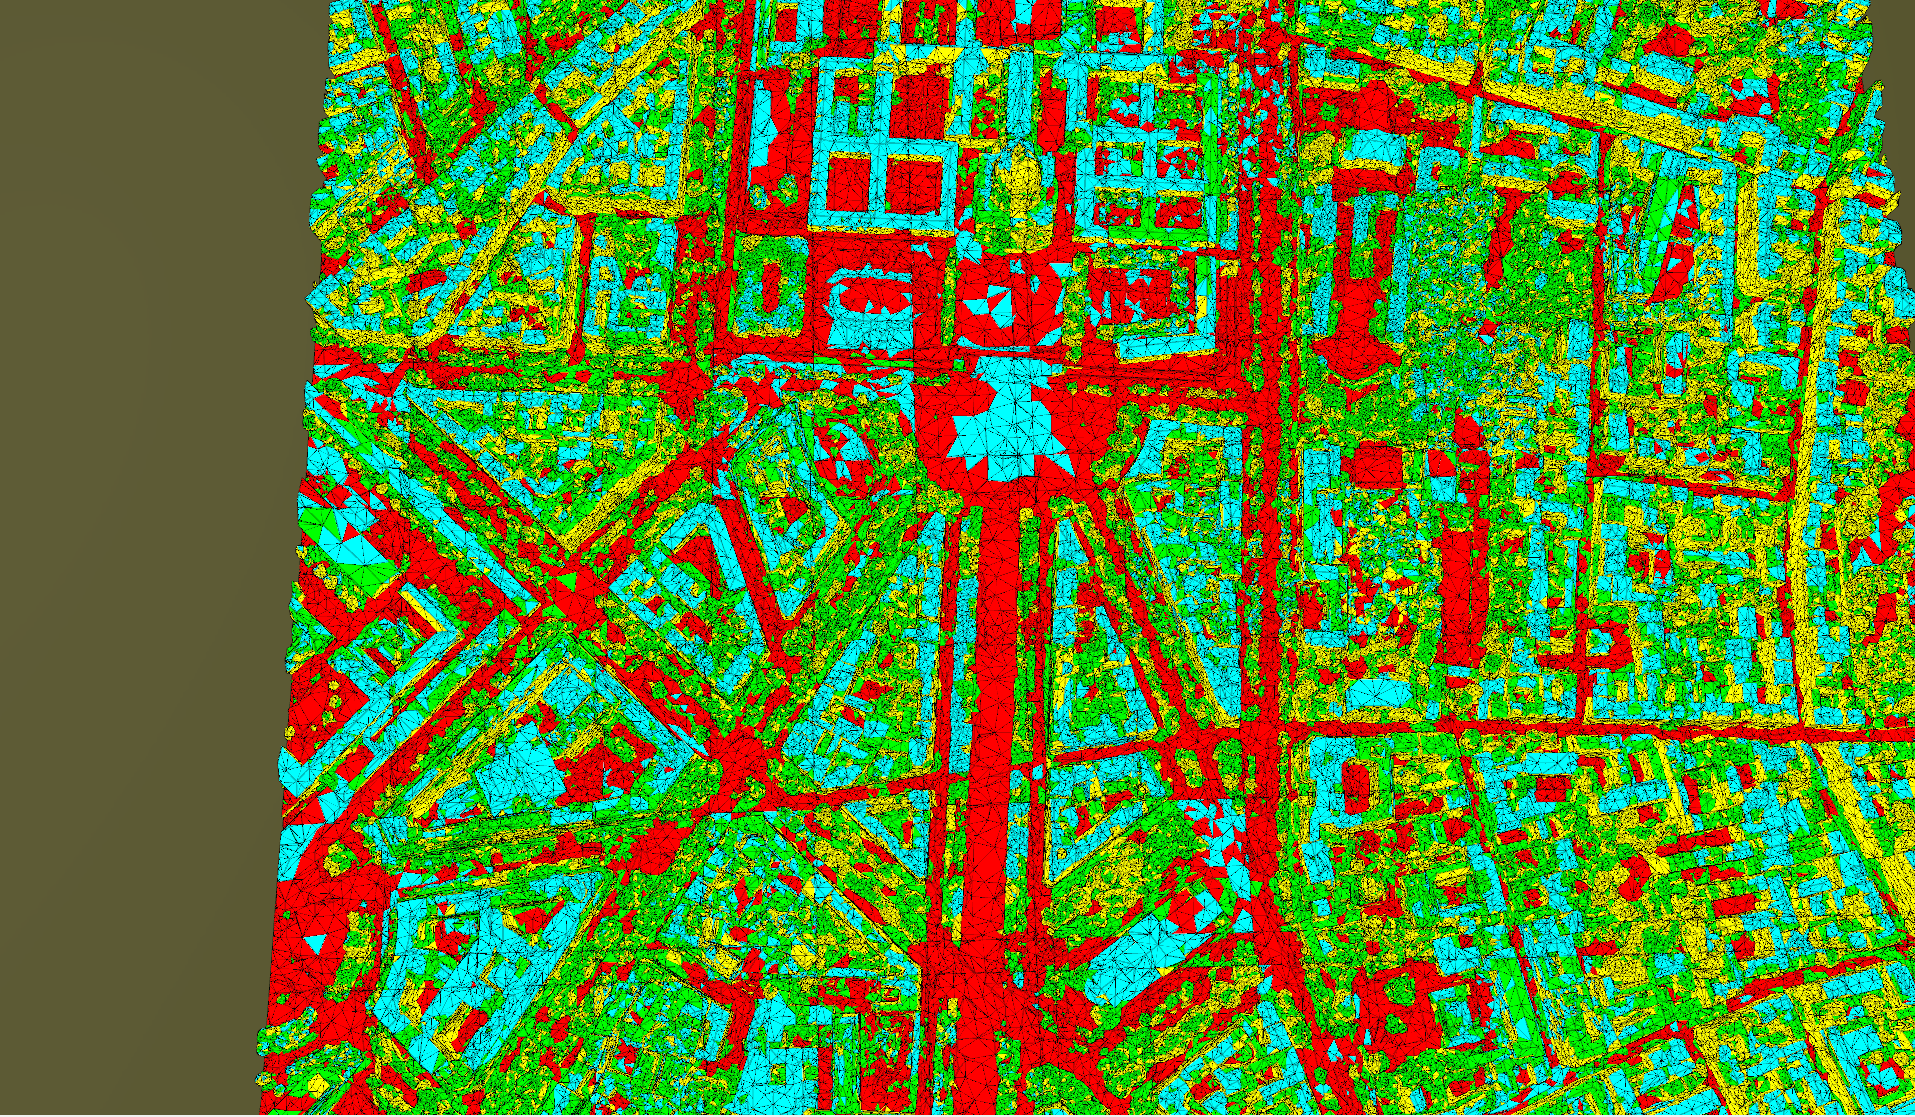
\includegraphics[width=0.9\textwidth]{images/MRF_res/paris_4class_verdie.png}
    \caption{Verdie orginal four-class-MRF formulation on Paris dataset}
    \label{fig:paris_verdie_mrf4}
\end{figure}
\begin{figure}[H]
    \centering
    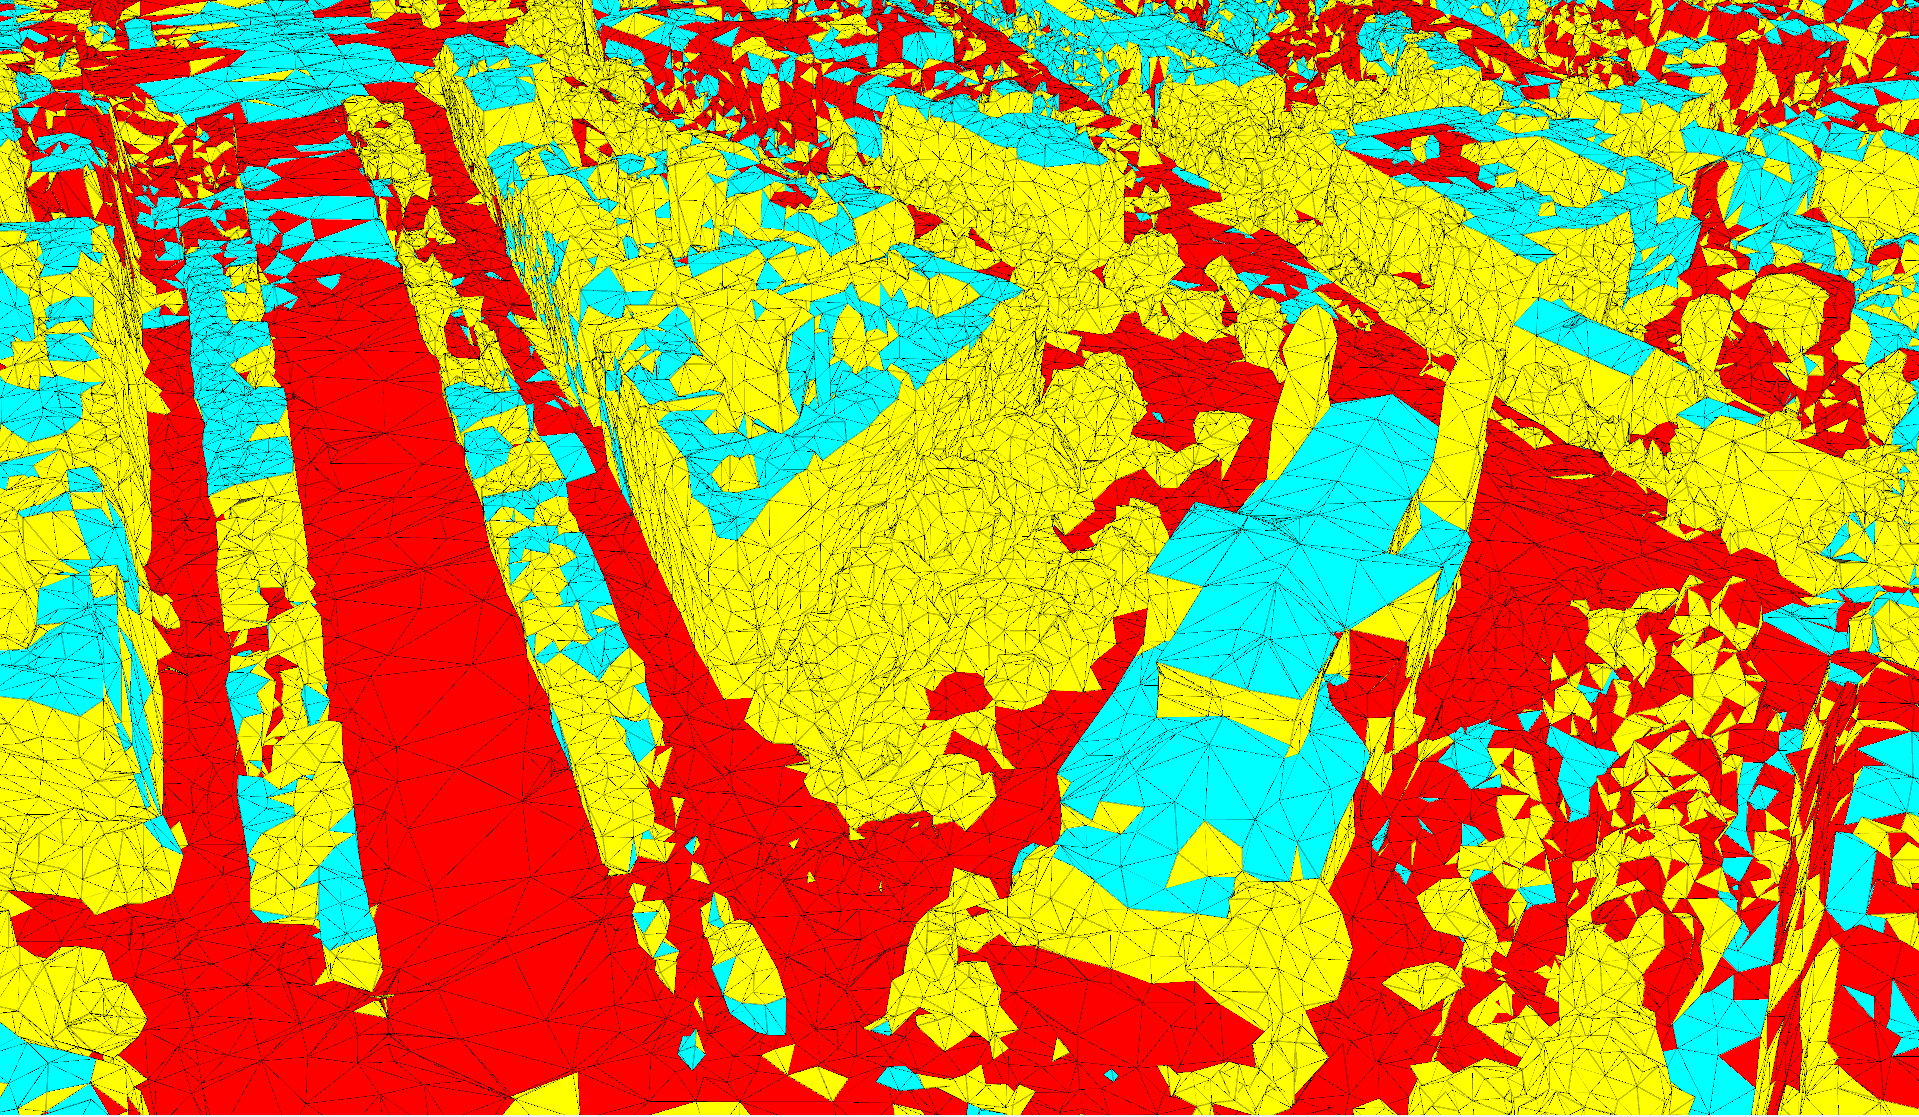
\includegraphics[width=0.9\textwidth]{images/MRF_res/paris_3class_verdie.png}
    \caption{Verdie three-class-MRF formulation on Paris dataset}
    \label{fig:paris_verdie_mrf3}
\end{figure}
 
\subsection{Object identification}
Textures comparison is a good compromise with limited resources and hilly grounds but is definitely far from optimal. The results are presented on Fig.~\ref{fig:object_detection_global} and Fig.~\ref{fig:object_detection_closeup} (local maxima are represented by red spheres). \\
In Fig.~\ref{fig:object_detection_closeup}, the  two main types of objects detected through the method are represented: ground objects, such as cars or bumps in the ground representation and segments from façades or low roofs, coming mostly from maxima present on the edge of the ground mesh. \\
The classification steps would then cluster these results from an automatic processing point of view, which corresponds to flattening the objects closer to the ground while leaving the higher ones intact. 
\begin{figure}[H]
    \centering
    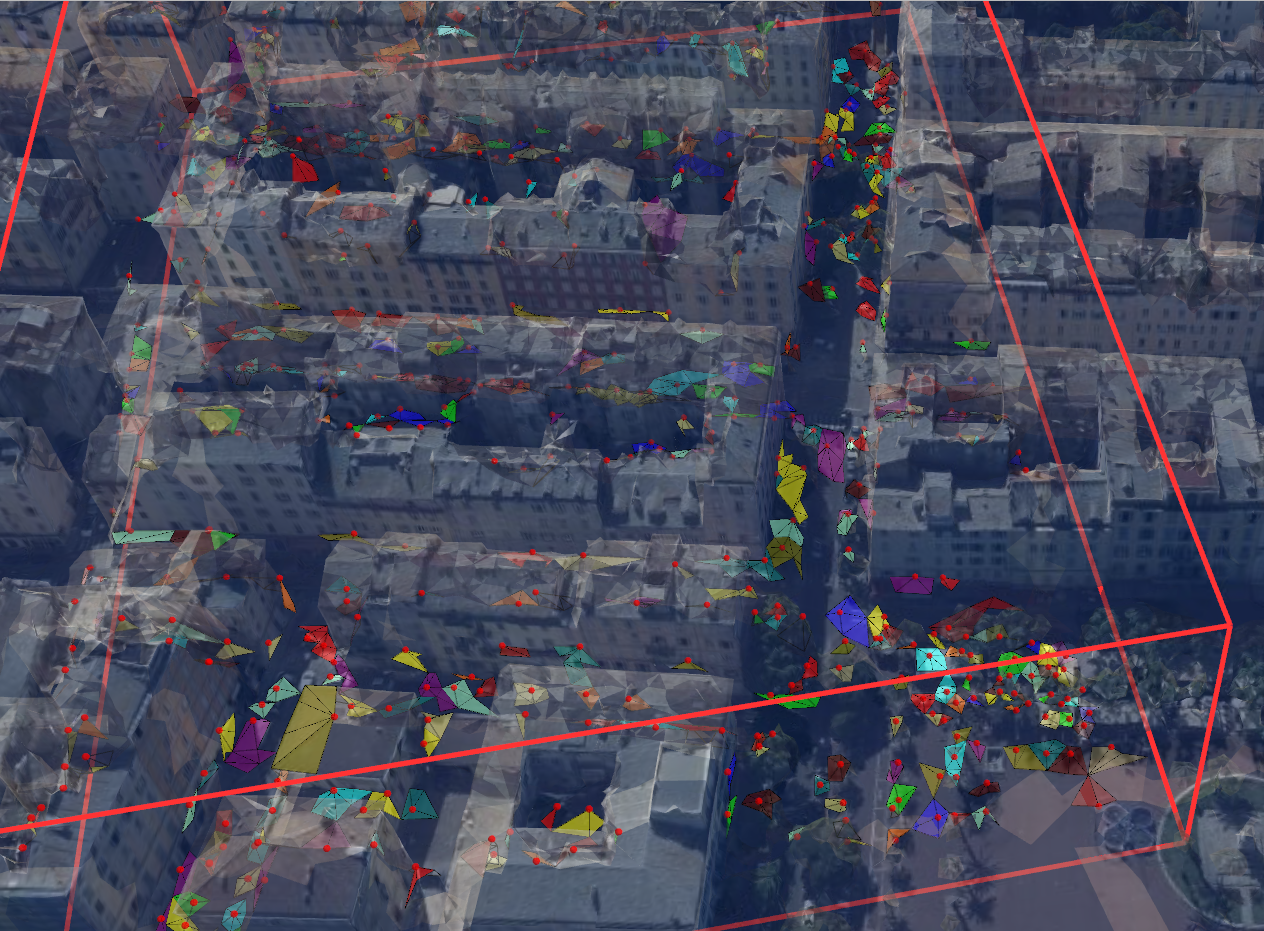
\includegraphics[width=0.9\textwidth]{images/Object_res/objects_from_local_maxima.png}
    \caption{Object detection: object detection in Bastia}
    \label{fig:object_detection_global}
\end{figure}
\begin{figure}[H]
    \centering
    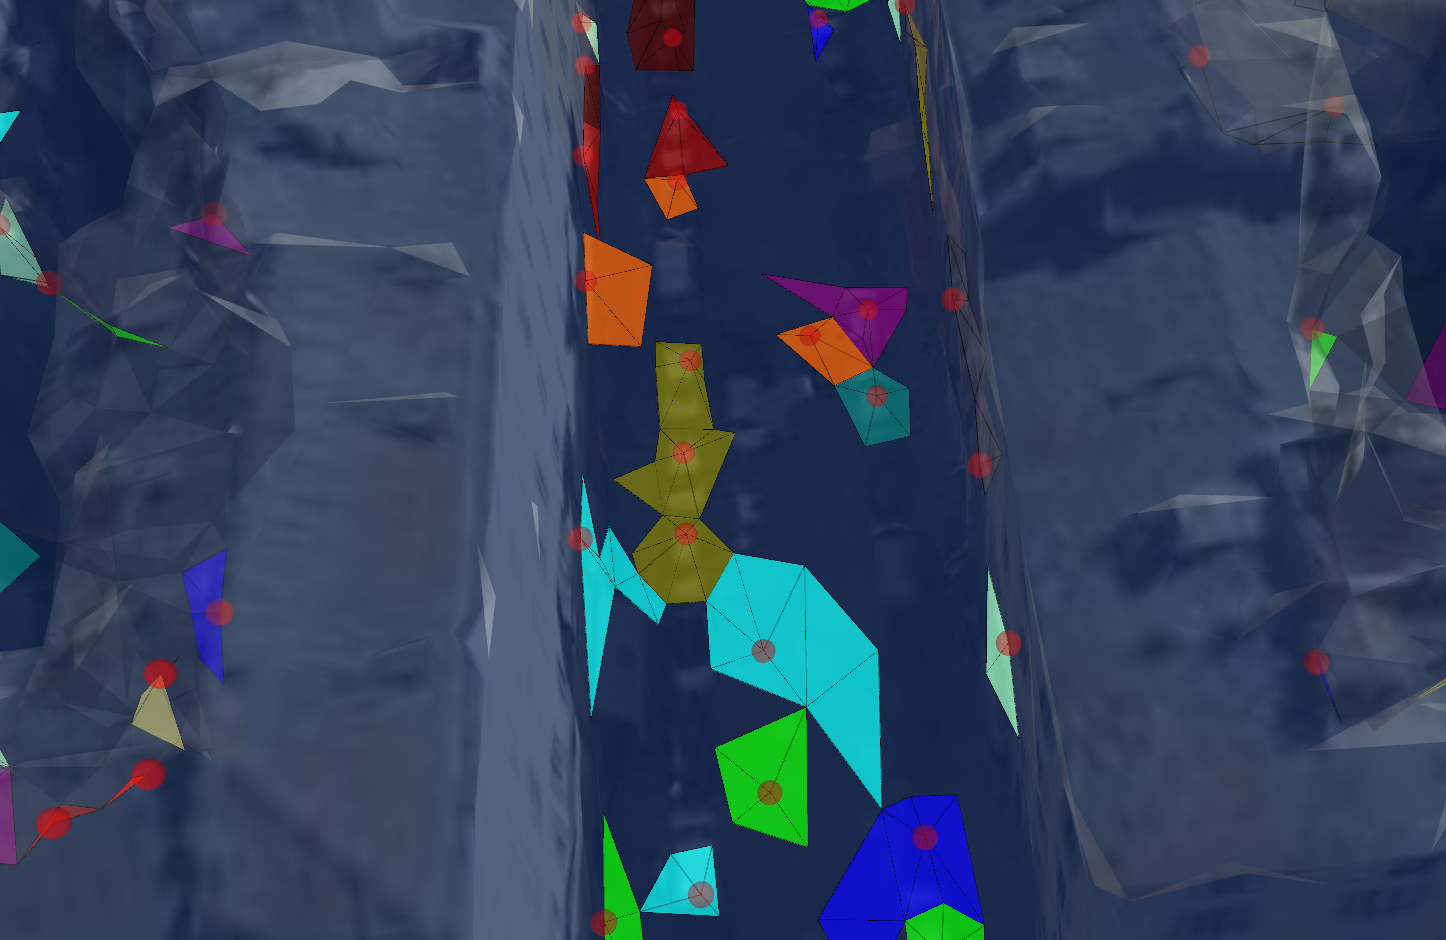
\includegraphics[width=0.9\textwidth]{images/Object_res/types_of_objects_detected.png}
    \caption{Object detection: types of detected objects}
    \label{fig:object_detection_closeup}
\end{figure}


\subsection{Conclusion}
On ideal cases, k-means and the MRF formulation perform quite similarly for three classes-identification. The fourth class, vegetation, identification requires further improvement using a MRF formulation, while usually leading to a split in the façade class when using k-means.  As k-means performs a clustering based on distance in the feature space, this is not surprising and this clustering behaviour is even more striking when classifying non-representative segments. \\
The suggested algorithm still faces most of the issues presented in \textcite{rouhani, verdie}: misclassification of ground as roof or façade in large flat areas. When using \textcite{verdie} unsupervised approach on lower resolution meshes, vegetation identification fails most of the time and calls for new, more discriminative features such as density-based suggestions. \\ 
As a general conclusion, the detection of artefacts in meshes is a rather complicated but solvable problem, on both higher and lower resolution meshes. The resolution however has to be high enough so that information is contained in geometric properties of the mesh rather than only in textures.  

\chapter{Discussion}
\section{Degree project limitations}
Several problems and constraints arose due to the degree project constraints. The first was that the investigated problem was shaped according to the available and usable data at Carmenta. This means that neither ground-truths nor detailed-enough elevation data were usable in association with the available data in the short time span of the project. Time evidently represented a constraint as well, as some results and suggestions presented in the algorithm were not included in the final results, such as effectively including the density feature in the MRF formulation. Finally, more on the engineering constraints, various approximations in computations arose due to the structure and format of the mesh data. 
\section{Future works}
Density holds potential for vegetation detection in meshes with varying resolutions. Due to time constraints, it was however not possible to effectively include it in the final proposal. As vegetation processing for artefact removal is usually rather specific, carrying on to a better-performing vegetation detection in the primary clustering via MRF step, it is important for the primary clustering to efficiently distinguish ground, buildings and trees. \\
In order to improve object detection, using available and accurate elevation data could allows to perform watershed without requiring texture-based constraints. Finally, in general, constituting ground-truths for supervised approach or simply performance evaluation could be of great benefit. 
\section{Conclusion}
From an engineering point of view, artefacts identification in urban meshes is a solvable problem. Given results and works on the detection of artefacts in 3D point clouds and that urban meshes are usually generated from point cloud surveying, it feels like performing such a detection step for quality purposes should be performed beforehand. \\
However, given a mesh, semantic segmentation is a relevant challenge for automatic simplification of the given mesh or for other applications. 
\section{Ethical and societal aspects}
Improving an urban model's quality by removing artefacts allows faster processing of the data which can be used towards efficient rescue missions planning. Digital models also play a very important in urban planning, allowing to visualise and anticipate risks through accurate simulations, as well as mitigating climate change and improving energy-efficiency as performed with the Helsinki data: paired with other energy-consumption-related sources, the model helps examine the solar energy potential of buildings. 


\printbibliography[heading=bibintoc] % Print the bibliography (and make it appear in the table of contents)

% \appendix






\end{document}
